\documentclass[11pt]{article} \usepackage{fullpage} \usepackage{graphicx} \usepackage{epstopdf} \usepackage{color} \usepackage{psfrag} \usepackage{pdfsync}\usepackage{indentfirst}\usepackage{subfigure}\usepackage{float}\usepackage[section]{placeins}
\usepackage{enumerate}
\usepackage{multirow}
\usepackage{amsfonts, fullpage, graphics} 
\usepackage{algorithm,algorithmic}
\usepackage{amsmath,amssymb,amsthm,bm,hyperref}
\usepackage{dsfont}
\usepackage[parfill]{parskip}
\usepackage[margin=1in]{geometry}
\newcommand{\Lagr}{\mathcal{L}}
\newcommand{\norm}[1]{\left\lVert#1\right\rVert}
\newcommand{\floor}[1]{\lfloor #1 \rfloor}
\newcommand{\todo}[1]{}
\renewcommand{\todo}[1]{{\color{red} TODO: {#1}}}
\newcommand\independent{\protect\mathpalette{\protect\independenT}{\perp}}
\newcommand{\obar}[1]{\mkern 1.5mu\overline{\mkern-1.5mu#1\mkern-1.5mu}\mkern 1.5mu}
\def\independenT#1#2{\mathrel{\rlap{$#1#2$}\mkern2mu{#1#2}}}
\newcommand{\rpm}{\sbox0{$1$}\sbox2{$\scriptstyle\pm$}
  \raise\dimexpr(\ht0-\ht2)/2\relax\box2 }
\usepackage{xspace}
\newcommand{\latex}{\LaTeX\xspace}
\setlength{\parindent}{2em}

\usepackage{listings}
\usepackage{color} %red, green, blue, yellow, cyan, magenta, black, white
\definecolor{mygreen}{RGB}{28,172,0} % color values Red, Green, Blue
\definecolor{mylilas}{RGB}{170,55,241}
\DeclareMathOperator{\E}{\mathbb{E}}
\DeclareMathOperator*{\argmax}{arg\,max}
\DeclareMathOperator*{\argmin}{arg\,min}

\begin{document}

{\parindent 0pt \begin{tabular}[t]{l} 16-720 Computer Vision \\ Spring 2020 \end{tabular}}%  \hfill XX/XX/14 \vskip 0.2in }
\parindent 0pt \parskip 8pt
\begin{center} \large\bf Homework 5 \end{center}
\begin{center} \large\bf Zongwen Mu, Andrew ID: zongwenm \end{center}
\bigskip


\section{Theory}

\setlength{\parindent}{2em}  

\paragraph{Q1.1}~{}

For each $x_i$ in vector $\bold{x}$, we have:
\begin{align}
	softmax\left(x_i\right) & = \frac{\mathrm{e}^{x_i}}{\begin{matrix} \sum_{j} \mathrm{e}^{x_j} \end{matrix}} \\
	softmax\left(x_i + c\right) & = \frac{\mathrm{e}^{x_i+c}}{\begin{matrix} \sum_{j} \mathrm{e}^{x_j+c} \end{matrix}} \\
	& = \frac{\mathrm{e}^{x_i}\mathrm{e}^{c}}{\begin{matrix} \sum_{j} \mathrm{e}^{x_j}\mathrm{e}^{c} \end{matrix}}  \\
	& = \frac{\mathrm{e}^{x_i}}{\begin{matrix} \sum_{j} \mathrm{e}^{x_j} \end{matrix}}
\end{align}

Therefore, $softmax(x) = softmax(x+c)$.

When $c = -\max{x_i}$, $x+c$ is always equal or less than $0$. This prevents explosion of exponential, so that the result won't overflow.

\paragraph{Q1.2}~{}

The range for each element is $\left(0, 1\right)$, the sum of all elements is $1$;

Softmax takes an arbitrary real valued vector $\bold{x}$ andand turns it into a probability distribution.

Calculating $s_i = \mathrm{e}^{x_i}$ is the outcome frequency in exponential form, $\mathbf{S} = \sum s_i$ calculates the total frequency, and dividing each $s_i$ by $\mathbf{S}$ normalizes the frequency of each $x_i$ and gets the probabilty.

\paragraph{Q1.3}~{}

When passing through fully connect layers, we have:
\begin{equation}
	y_i = W_ix_i + b_i
\end{equation}

Therefore, when applying multi-layer, we have:
\begin{align}
	y_n & = W_nx_n + b_n \\
	& = W_n\left(W_{n-1}x_{n-1} + b_{n-1}\right) + b_n \\
	& = W_nW_{n-1}x_{n-1} + W_nb_{n-1} + b_n \\
	& = W^\prime x_{n-1} + b^\prime \\
	& \cdots \\
	& = Wx + b
\end{align}

which is same as linear regression problem.

\paragraph{Q1.4}~{}

Derivative of $\sigma\left(x\right)$:
\begin{align}
	\frac{\mathrm{d}}{\mathrm{d}x}\sigma(x) & = \frac{\mathrm{d}}{\mathrm{d}x}\left(1 + \mathrm{e}^{-x}\right)^{-1} \\
	& = \frac{\mathrm{e}^{-x}}{\left(1+\mathrm{e}^{-x}\right)^{2}} \\
	& = \frac{1}{1+\mathrm{e}^{-x}}\frac{1+\mathrm{e}^{-x}-1}{1+\mathrm{e}^{-x}} \\
	& = \sigma(x) \left[1 - \sigma(x)\right]
\end{align}

\paragraph{Q1.5}~{}

\begin{align}
	y & = Wx + b \\
	\frac{\partial J}{\partial W} & = \frac{\partial J}{\partial y}\frac{\partial y}{\partial W} \\
	& = \delta x^\mathrm{T} \\
	\frac{\partial J}{\partial x} & = \frac{\partial J}{\partial y}\frac{\partial y}{\partial x} \\
	& = W^\mathrm{T}\delta \\
	\frac{\partial J}{\partial b} & = \frac{\partial J}{\partial y}\frac{\partial y}{\partial b} \\
	& = \delta
\end{align}

\paragraph{Q1.6}~{}

1. The derivative of sigmoid function is range in $\left(0, 0.25\right)$, which is rather small. Therefore, when applied in multiple layers, it may cause "gradient vanish".

2. The output range of sigmoid function is $\left(0, 1\right)$, while the output range of tanh function is $\left(-1, 1\right)$. Tanh function is preferred because it could reach the negative part when $x$ is negative.

3. The derivative of tanh function has a range of $\left(0, 1\right)$, therefore, the gradient would drop slower and is less likely to cause gradient vanish compared with sigmoid function.

4. 
\begin{align}
	\sigma(x) & = \frac{1}{1+\mathrm{e}^{-x}} \\
	\frac{1-\mathrm{e}^{-x}}{1+\mathrm{e}^{-x}} & = 2\sigma(x) - 1 \\
	tanh(x) & = \frac{1-\mathrm{e}^{-2x}}{1+\mathrm{e}^{-2x}} \\
	& = 2\sigma(2x) - 1
\end{align}

\section{Implement a Fully Connected Network}
\subsection{Network Initialization}

\paragraph{Q2.1.1}~{}

Since we need to multiply the inputs of each layer by the weights, if the network is initialized with all zeros, the output from the network will all be zero, and the probabilities would all be the same.

\paragraph{Q2.1.3}~{}

Initializing the network with random numbers can avoid getting the same computations from each layer. Scaling the initialization depending on layer size could help keep the variance around desired values when doing forward and backwards propagation.

\section{Training Models}

\paragraph{Q3.1}~{}

With learning rate modified to $3e-3$, batch size set to $32$, after $100$ iterations, the valid accuracy is $76.25\%$. Since the valid loss is quite insignificant compared with training loss, so I averaged training loss by the number of samples, the loss and accuracy figures are shown below:
\begin{figure}[H]
\centering
\subfigure[Loss Figure]{
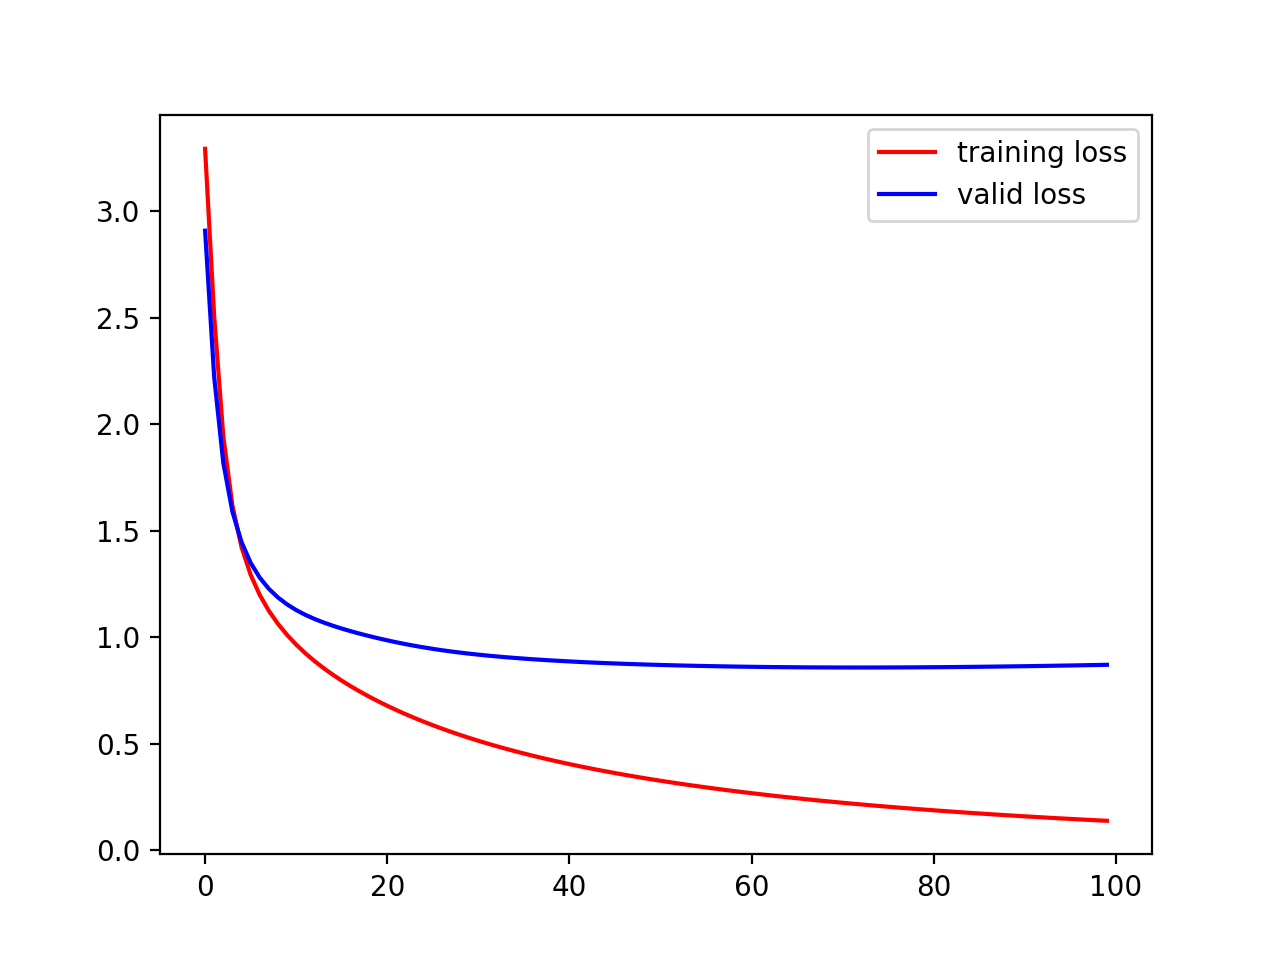
\includegraphics[width=0.4\textwidth]{results/q3_1_loss.png}}
\subfigure[Accuracy Figure]{
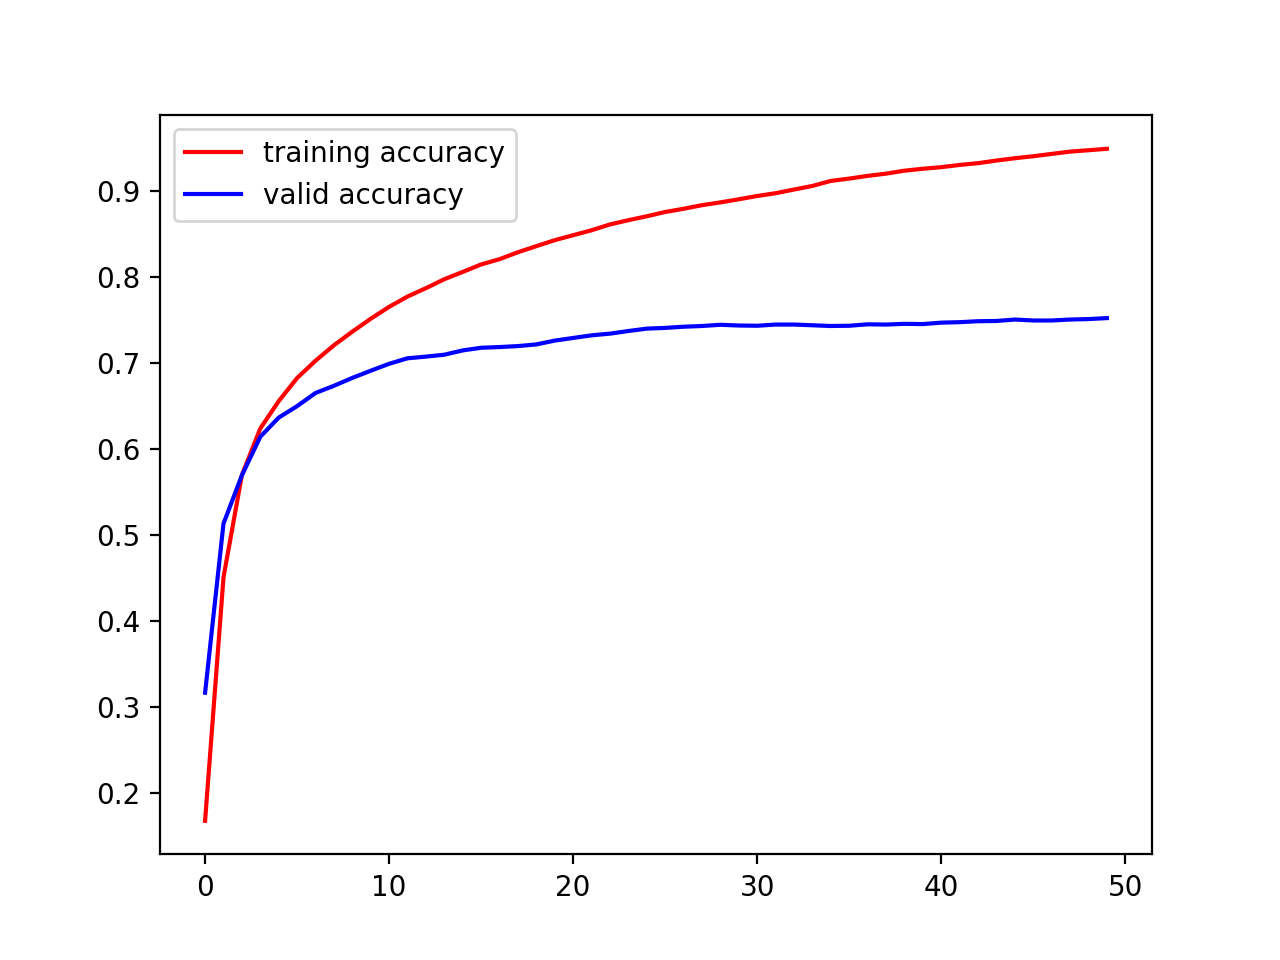
\includegraphics[width=0.4\textwidth]{results/q3_1_acc.png}}
\caption{Loss and Accuracy Figures}
\end{figure}

\paragraph{Q3.2}~{}
With learning rate $3e-2$, the figures are look like:
\begin{figure}[H]
\centering
\subfigure[Loss Figure]{
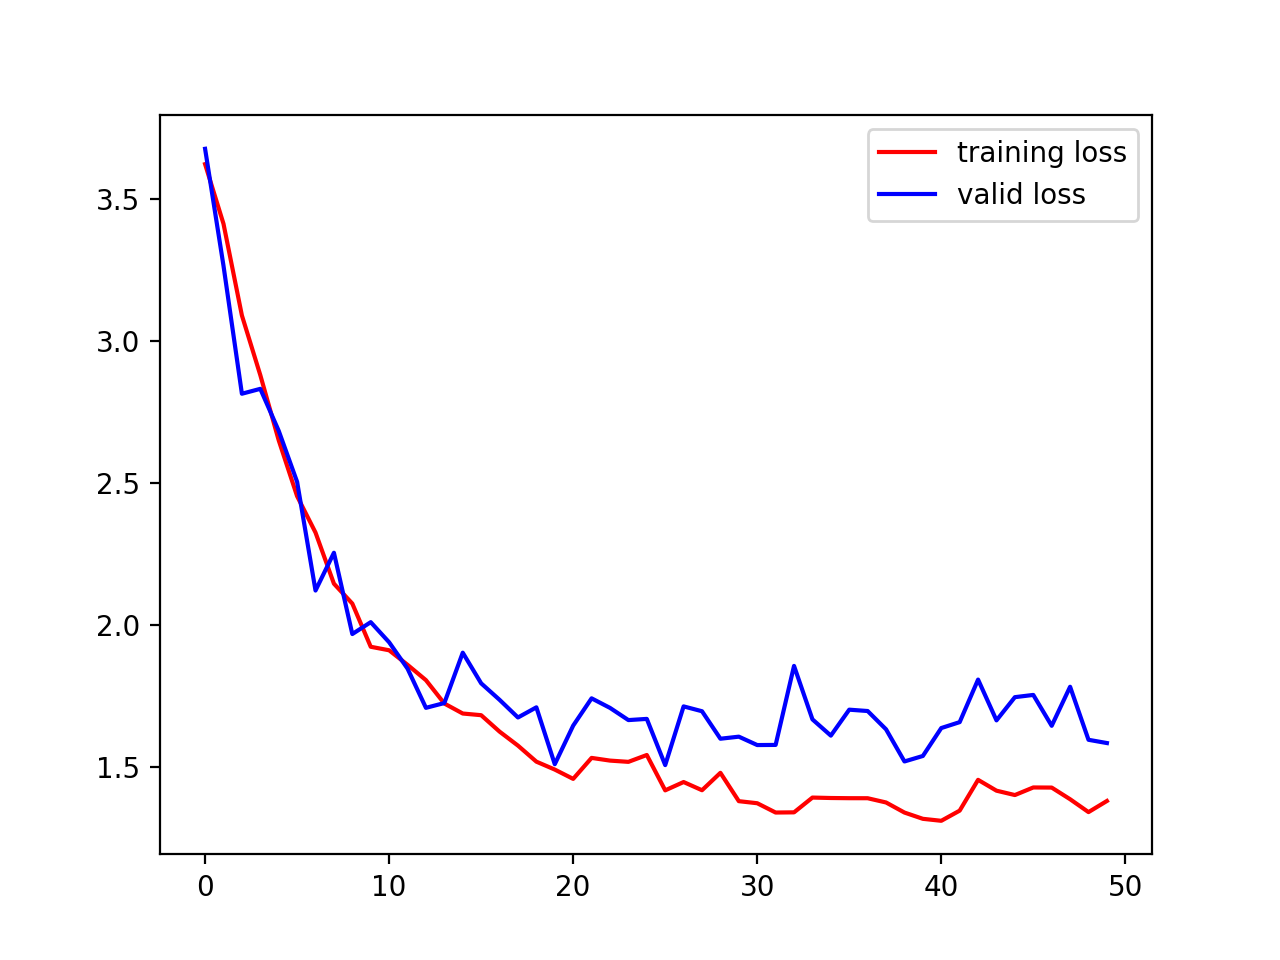
\includegraphics[width=0.4\textwidth]{results/q3_2_loss10.png}}
\subfigure[Accuracy Figure]{
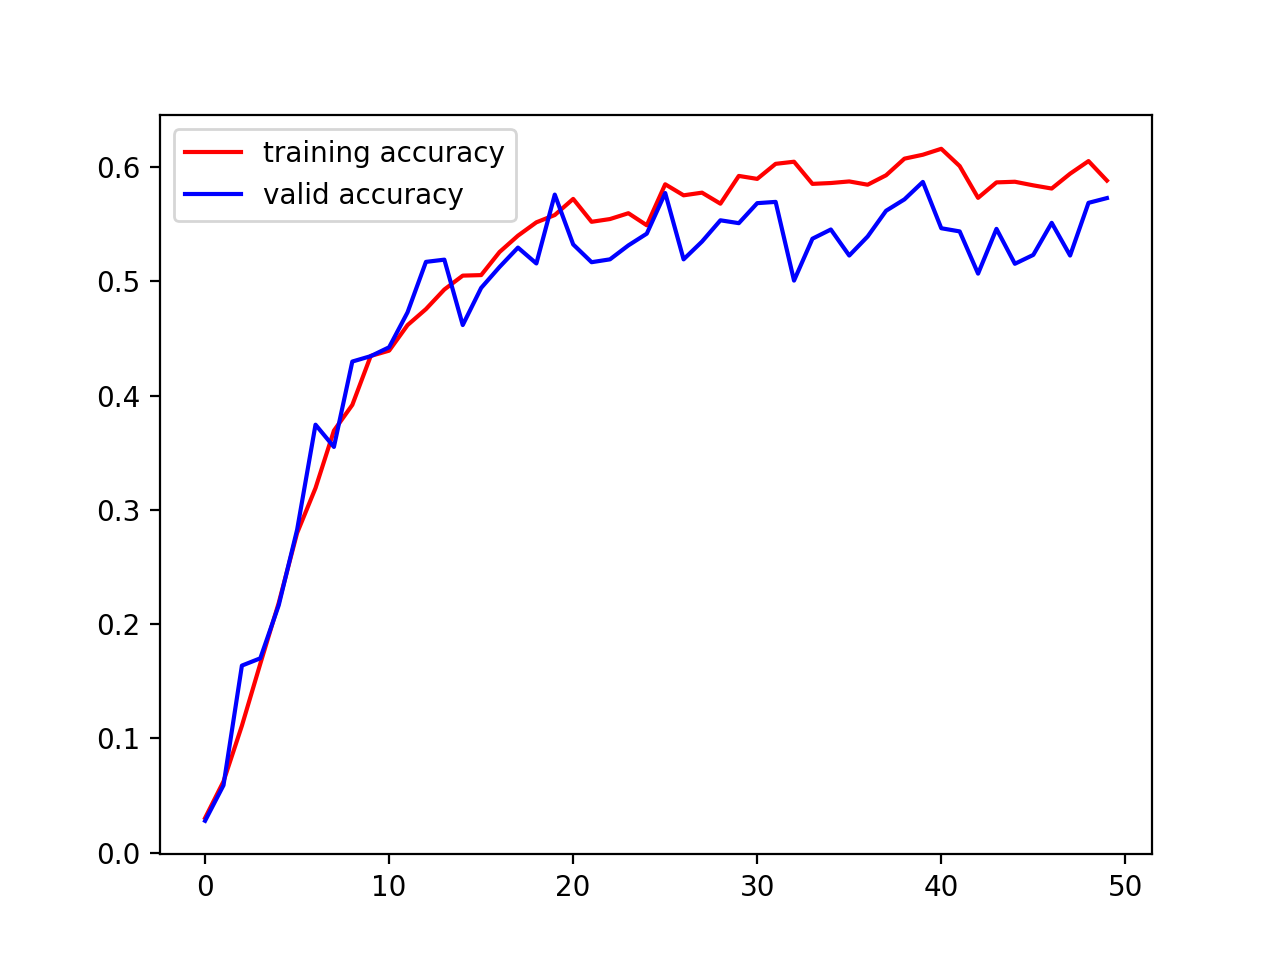
\includegraphics[width=0.4\textwidth]{results/q3_2_acc10.png}}
\caption{Loss and Accuracy Figures}
\end{figure}

The losses are higher and the accuracy dropped, and there is also oscillation occurred.

With learning rate $3e-4$, the figures are look like:
\begin{figure}[H]
\centering
\subfigure[Loss Figure]{
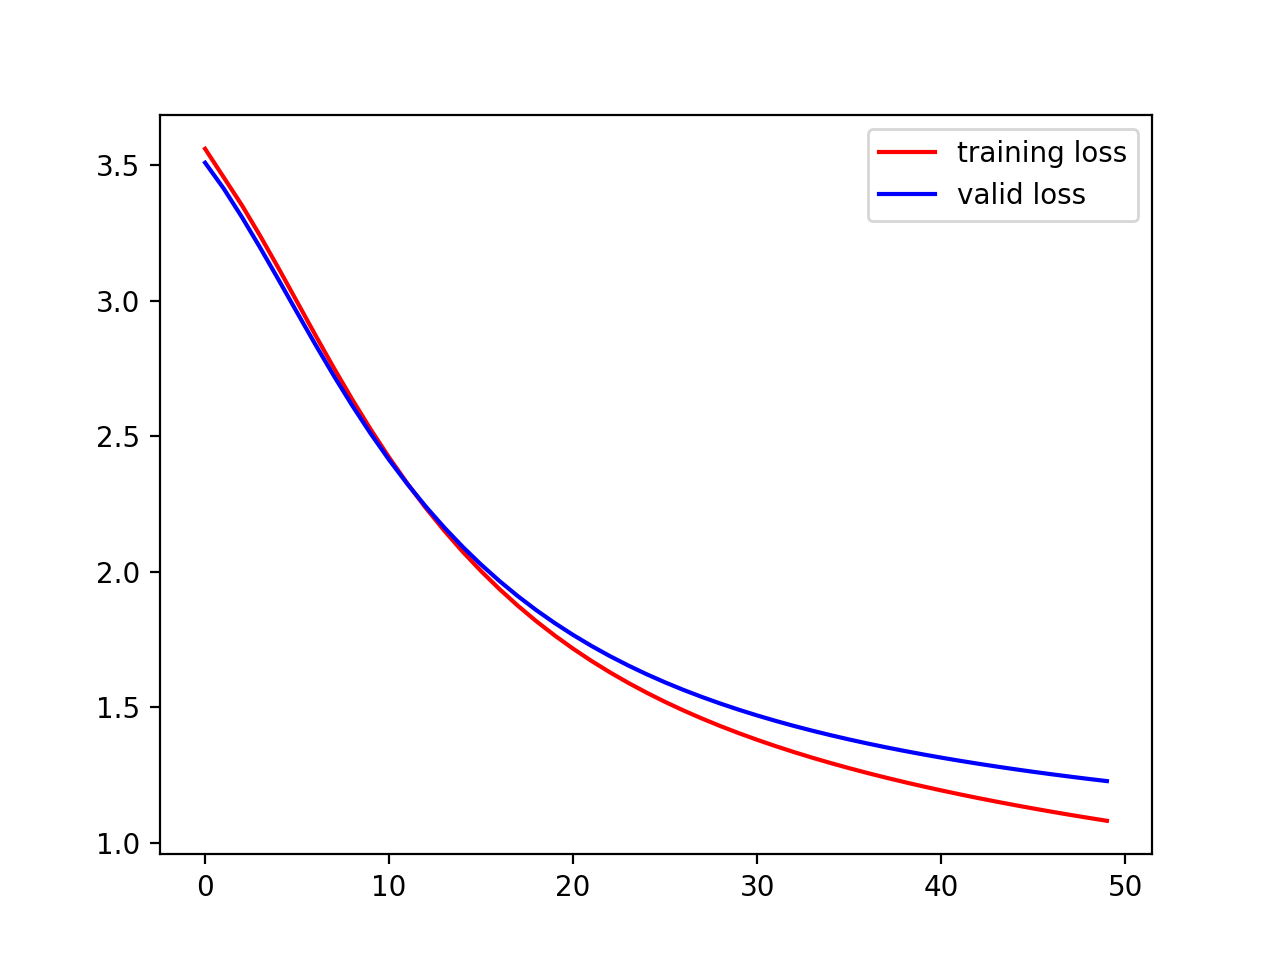
\includegraphics[width=0.4\textwidth]{results/q3_2_loss01.png}}
\subfigure[Accuracy Figure]{
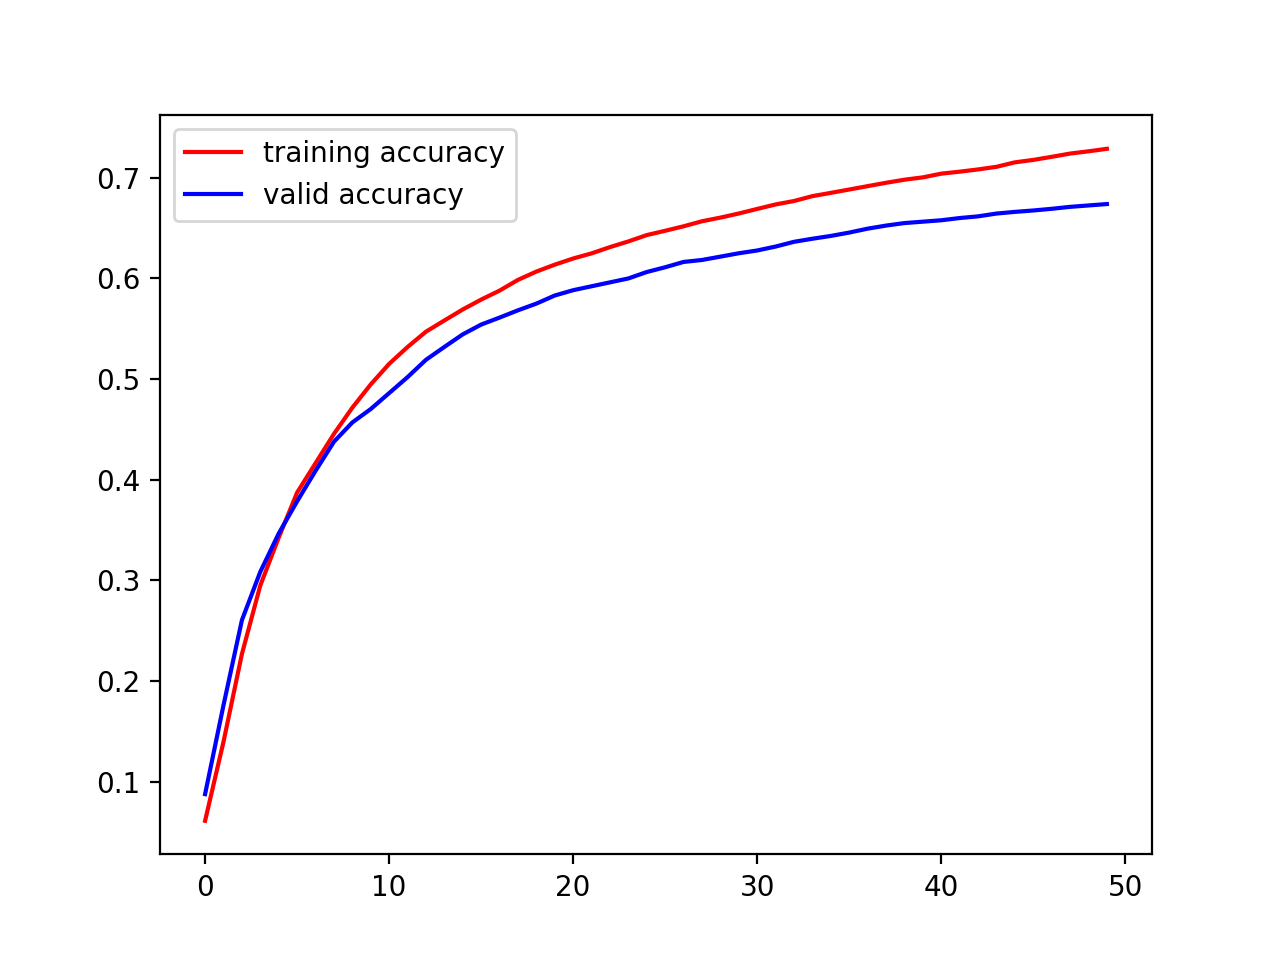
\includegraphics[width=0.4\textwidth]{results/q3_2_acc01.png}}
\caption{Loss and Accuracy Figures}
\end{figure}

The curves are smooth but since the step is too small, the network didn't converge to the optimum within the max iteration number $100$.

\paragraph{Q3.3}~{}

The visualization of the initialized first layer weights were shown below:
\begin{figure}[H]
\centering
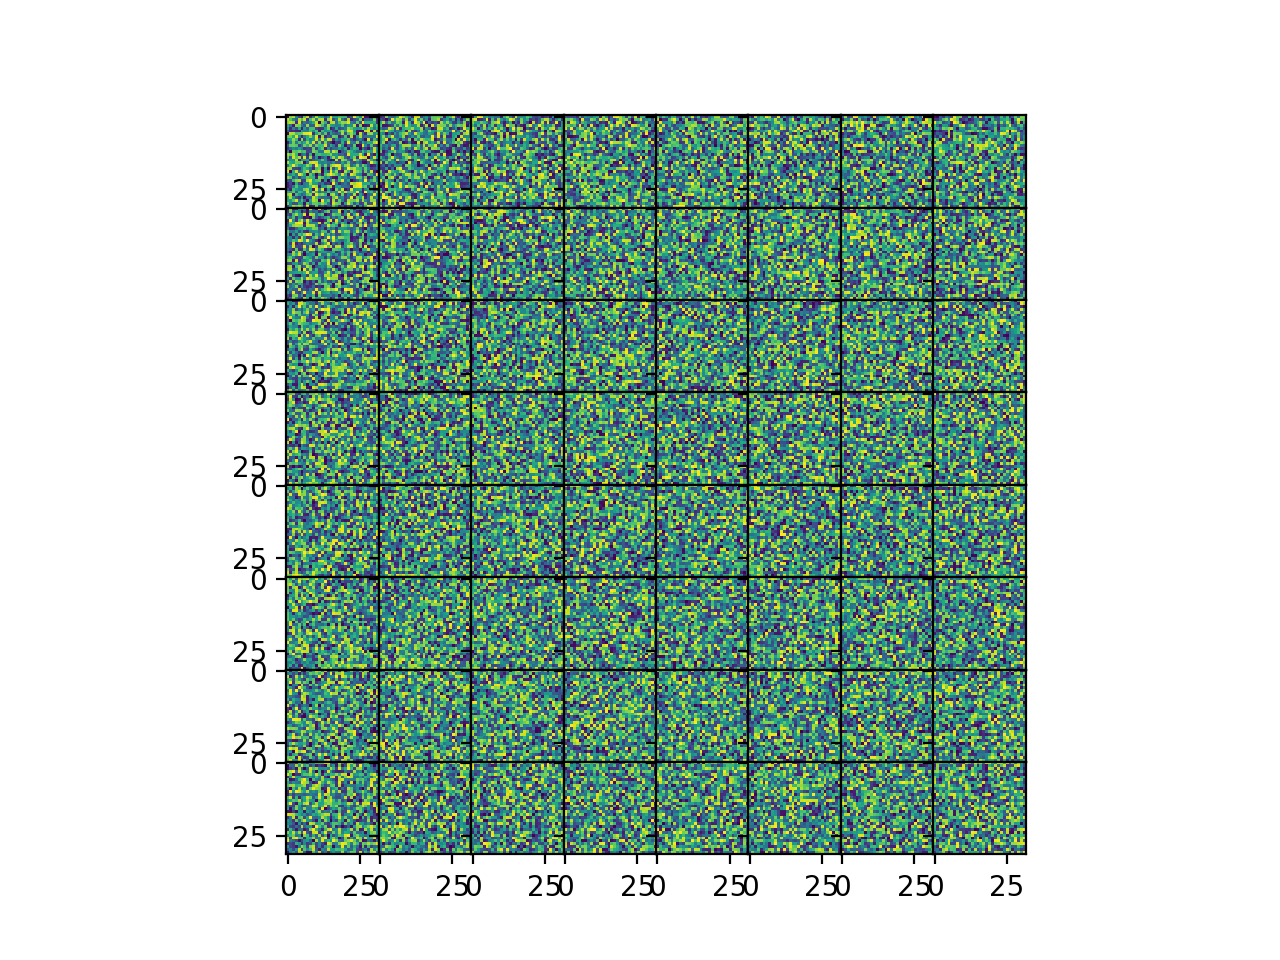
\includegraphics[width=0.7\textwidth]{results/q3_3_before.png}
\caption{Initialized Weights}
\end{figure}

The visualization of learned first layer weights were shown below:
\begin{figure}[H]
\centering
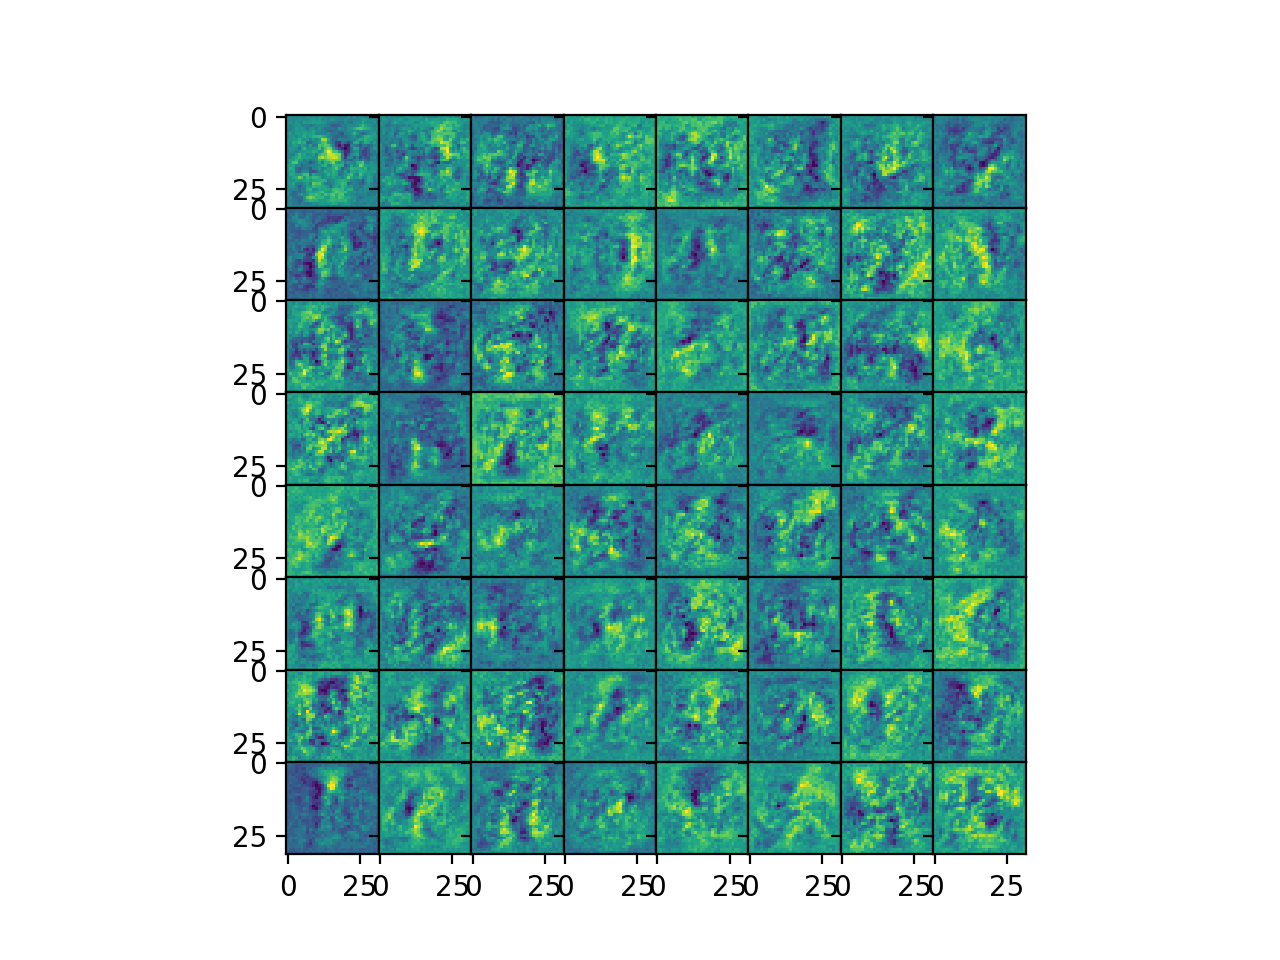
\includegraphics[width=0.7\textwidth]{results/q3_3_after.png}
\caption{Trained Weights}
\end{figure}

Comparing these two figures, we could find that the initialized weights look like random noise since we initialize the weights with random uniform distribution. After training, the learned weights are more clear patterns.

\paragraph{Q3.4}~{}

The visualized confusion matrix is shown below:
\begin{figure}[H]
\centering
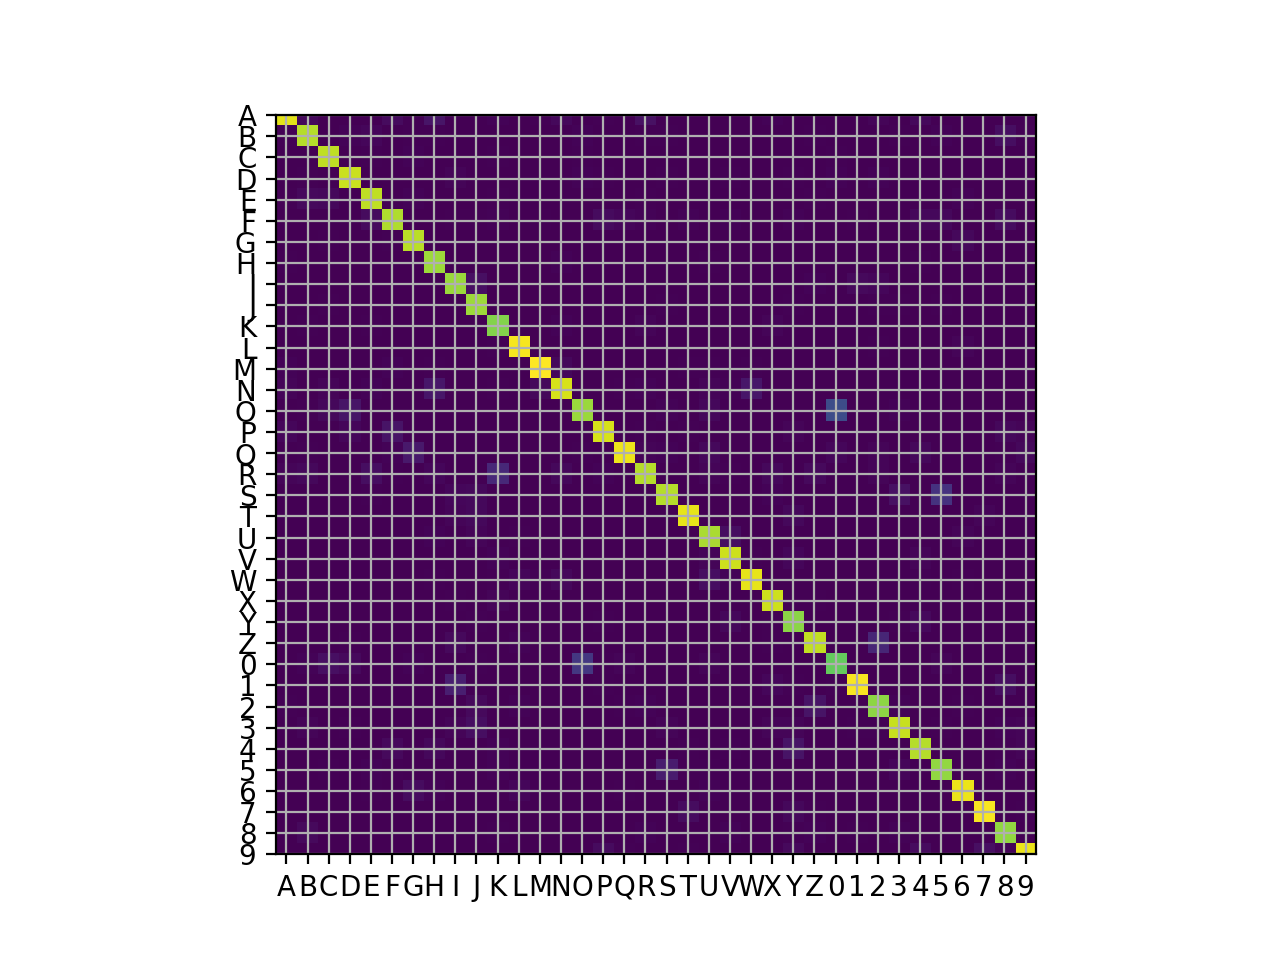
\includegraphics[width=0.8\textwidth]{results/q3_4.png}
\caption{Confusion Matrix}
\end{figure}

From the figure we can tell the most commonly confused pairs are: $`\mathrm{O}`$ and $`0`$, $`\mathrm{s}`$ and $`5`$, which have similar shape that would often be misjudged easily.

\section{Extract Text from Images}

\paragraph{Q4.1}~{}

The assumptions are:

1. Every letter is fully connected.

2. Two different letters are not connected.

Since we extract the letters by finding connected pixels, so if parts of the character are separated or there are several connected characters, it may cause error in detection.

Example images:
\begin{figure}[H]
\centering
\subfigure[Letter not fully connected]{
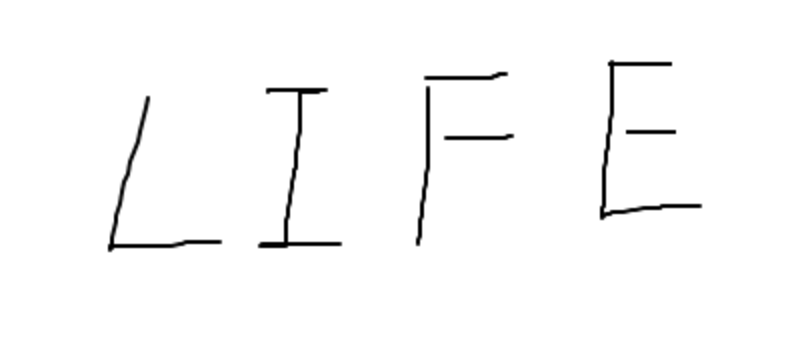
\includegraphics[width=0.4\textwidth]{results/q4_1_1.png}}
\subfigure[Connected letters]{
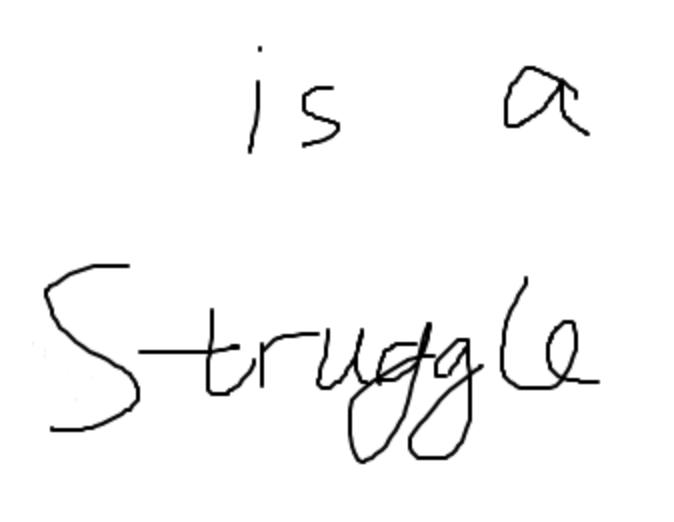
\includegraphics[width=0.4\textwidth]{results/q4_1_2.png}}
\caption{Examples of Possible Detection Failure}
\end{figure}

\paragraph{Q4.3}~{}

All letters were detected correctly, results are shown below:
\begin{figure}[H]
\centering
\subfigure[]{
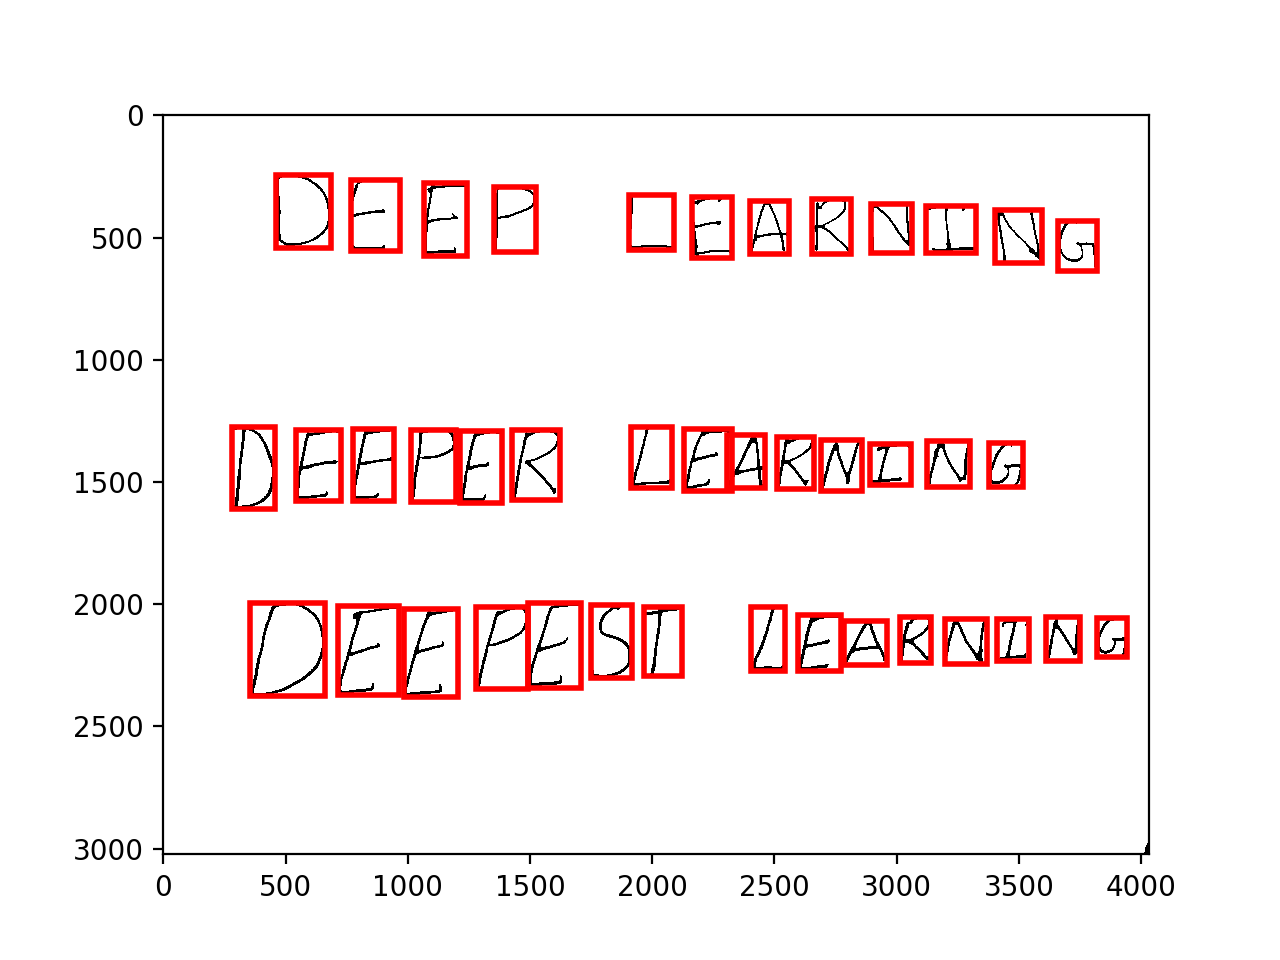
\includegraphics[width=0.4\textwidth]{results/q4_3_1.png}}
\subfigure[]{
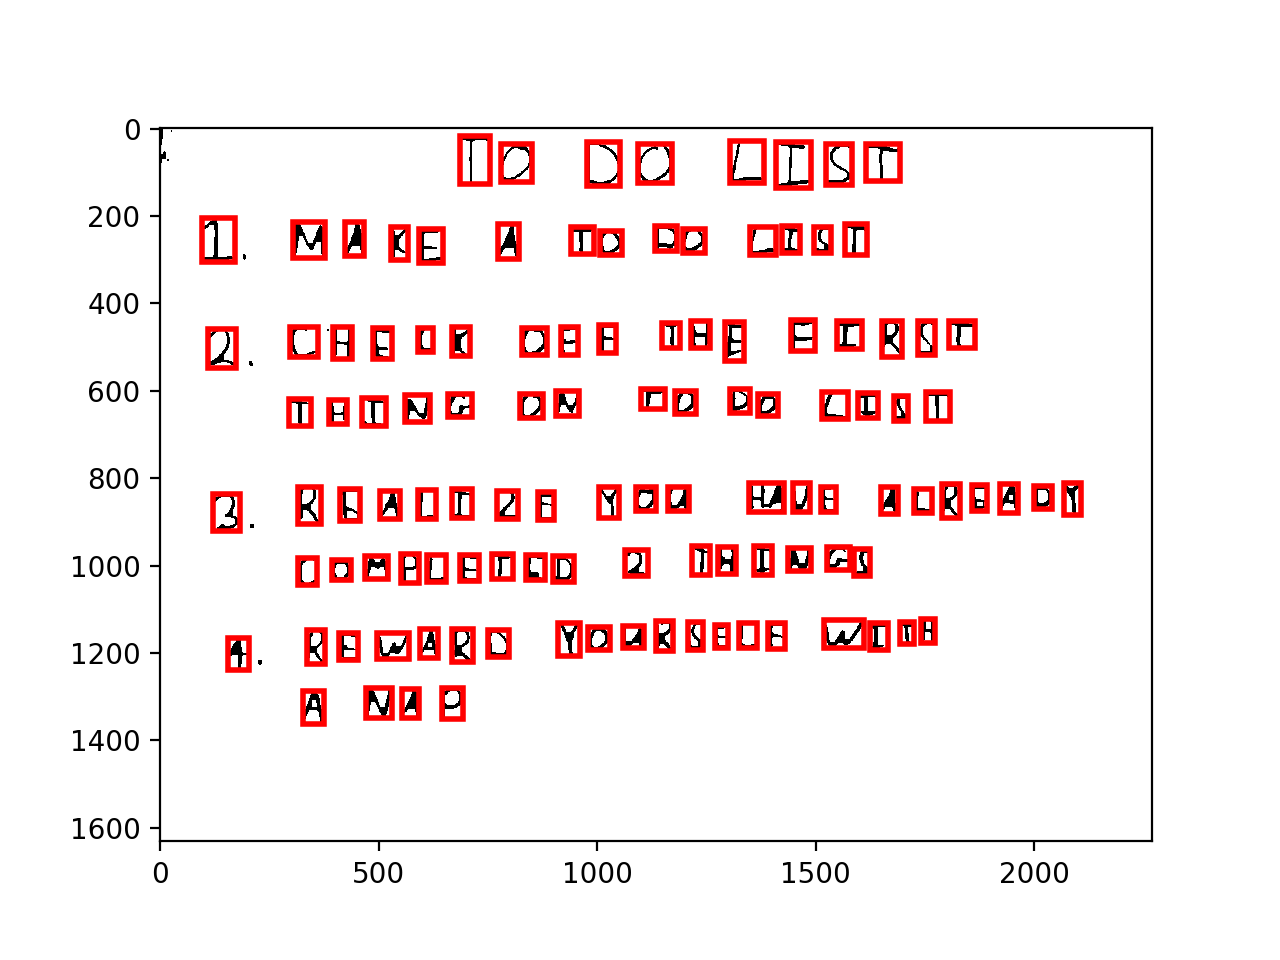
\includegraphics[width=0.4\textwidth]{results/q4_3_2.png}}
\subfigure[]{
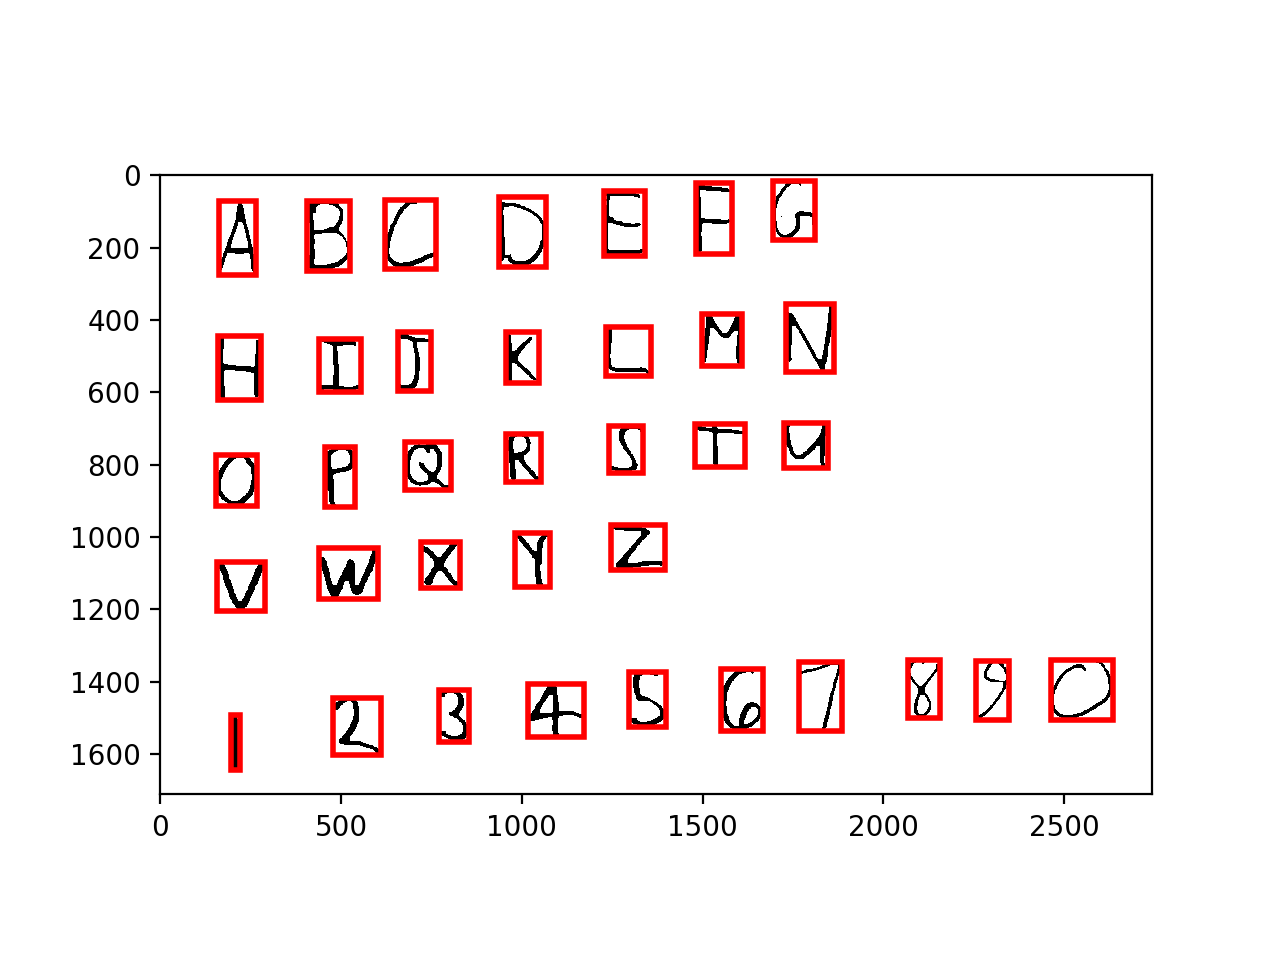
\includegraphics[width=0.4\textwidth]{results/q4_3_3.png}}
\subfigure[]{
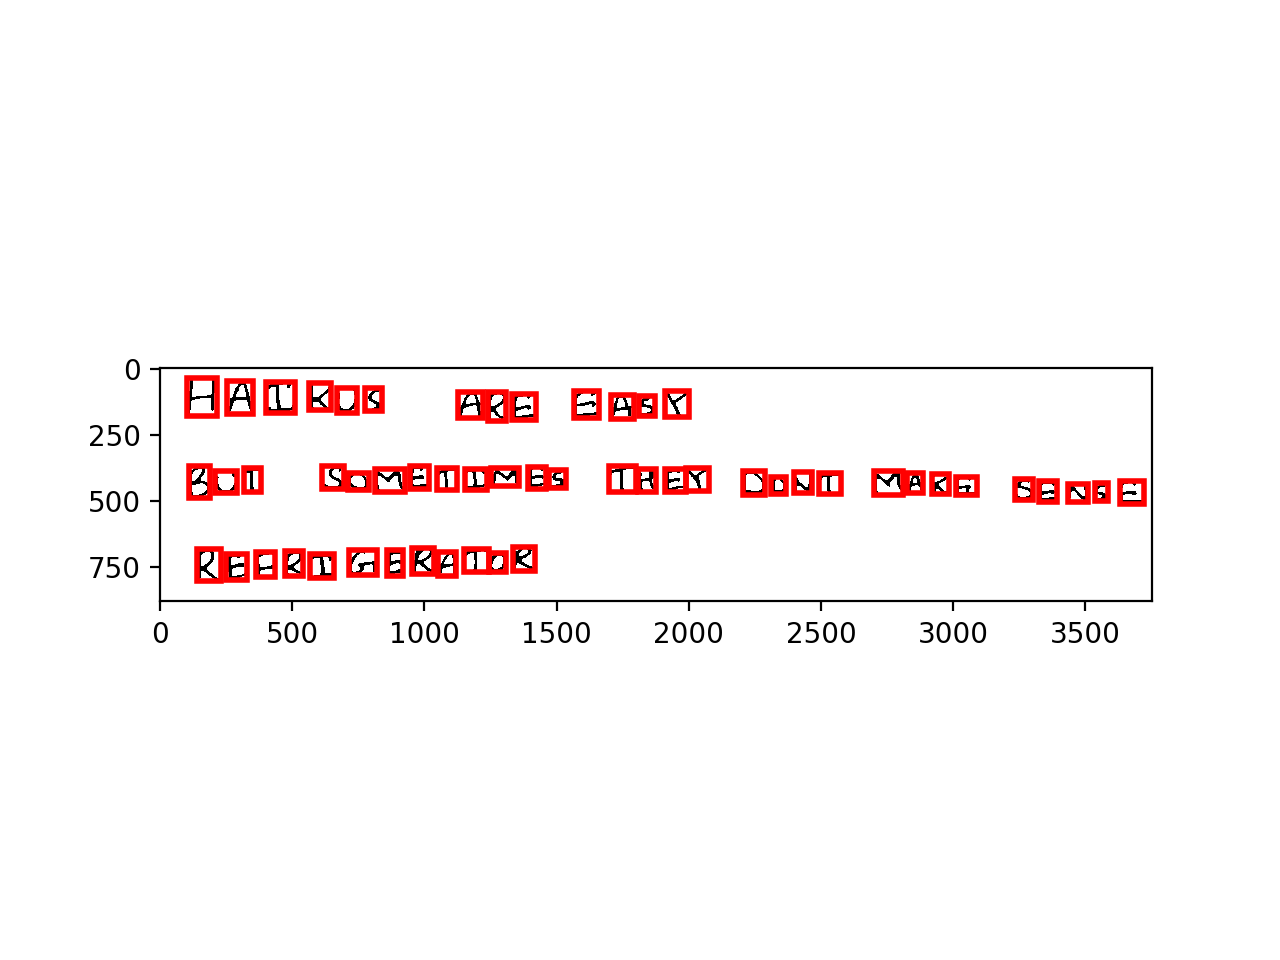
\includegraphics[width=0.4\textwidth]{results/q4_3_4.png}}
\caption{Detection Results}
\end{figure}

\section{Image Compression with Autoencoders}

\setcounter{subsection}{1}
\subsection{Training the Autoencoder}
\paragraph{Q5.2}~{}

With default settings and batch size $36$, learning rate $3e-5$, the loss curves are shown below:
\begin{figure}[H]
\centering
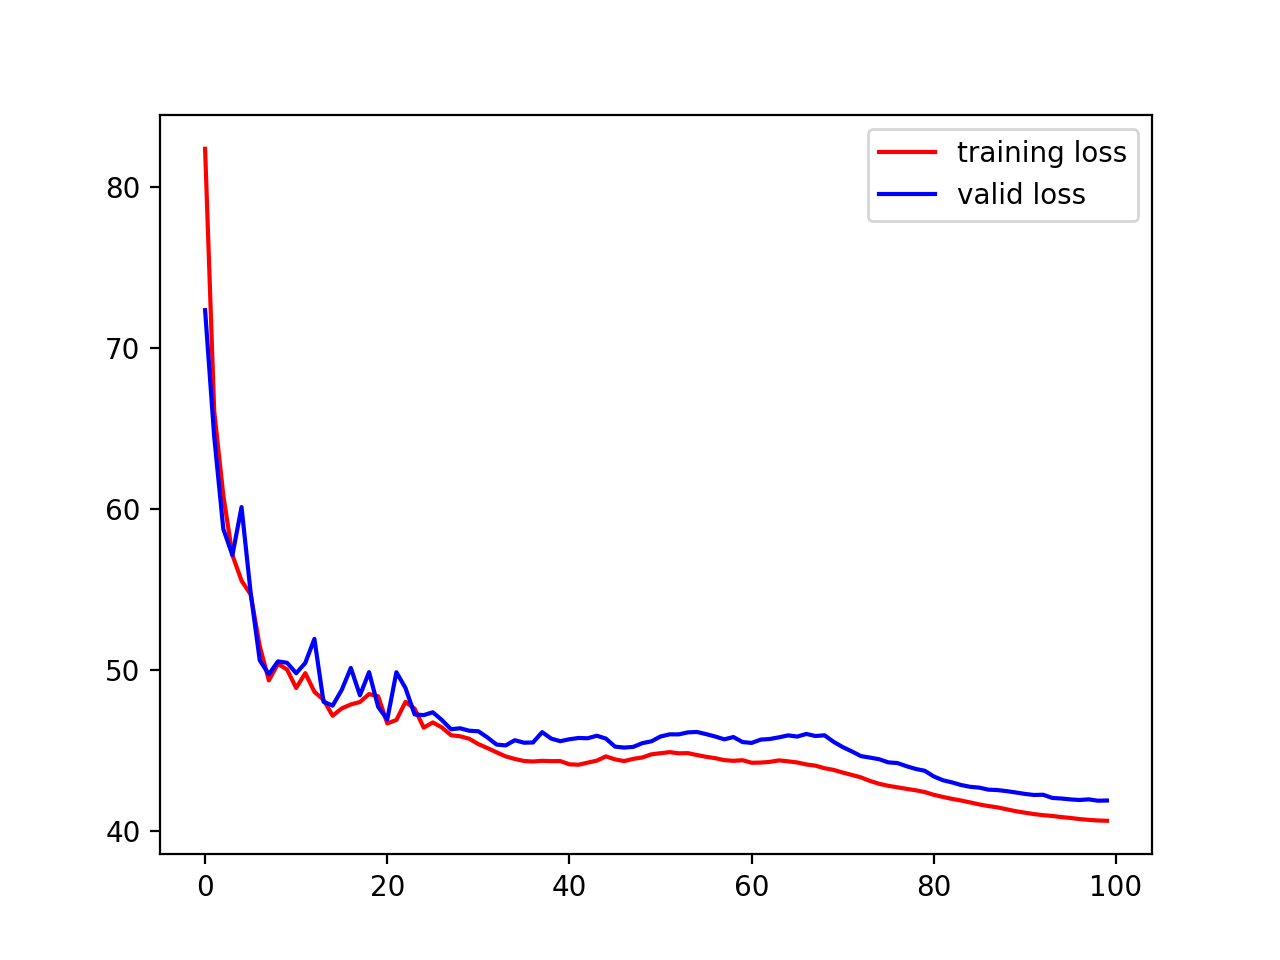
\includegraphics[width=0.8\textwidth]{results/q5_2_loss.png}
\caption{Loss Figure}
\end{figure}

As training epochs increase, the loss dropped in a vibrating way, but it became smoother at the end of training.

\subsection{Evaluating the Autoencoder}
\paragraph{Q5.3.1}~{}

Class $2$:
\begin{figure}[H]
\centering
\subfigure[]{
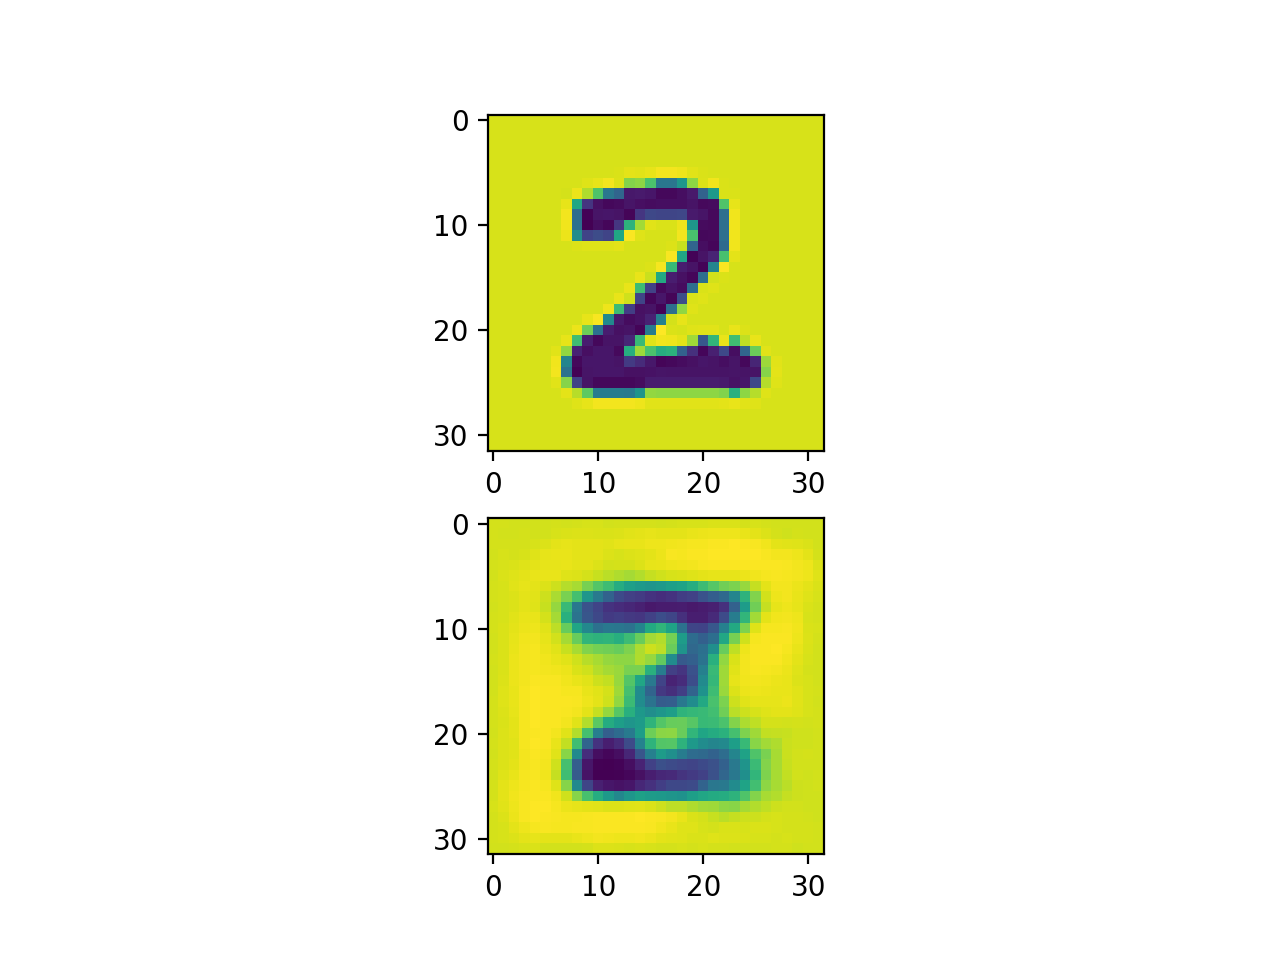
\includegraphics[width=0.4\textwidth]{results/q5_3_21.png}}
\subfigure[]{
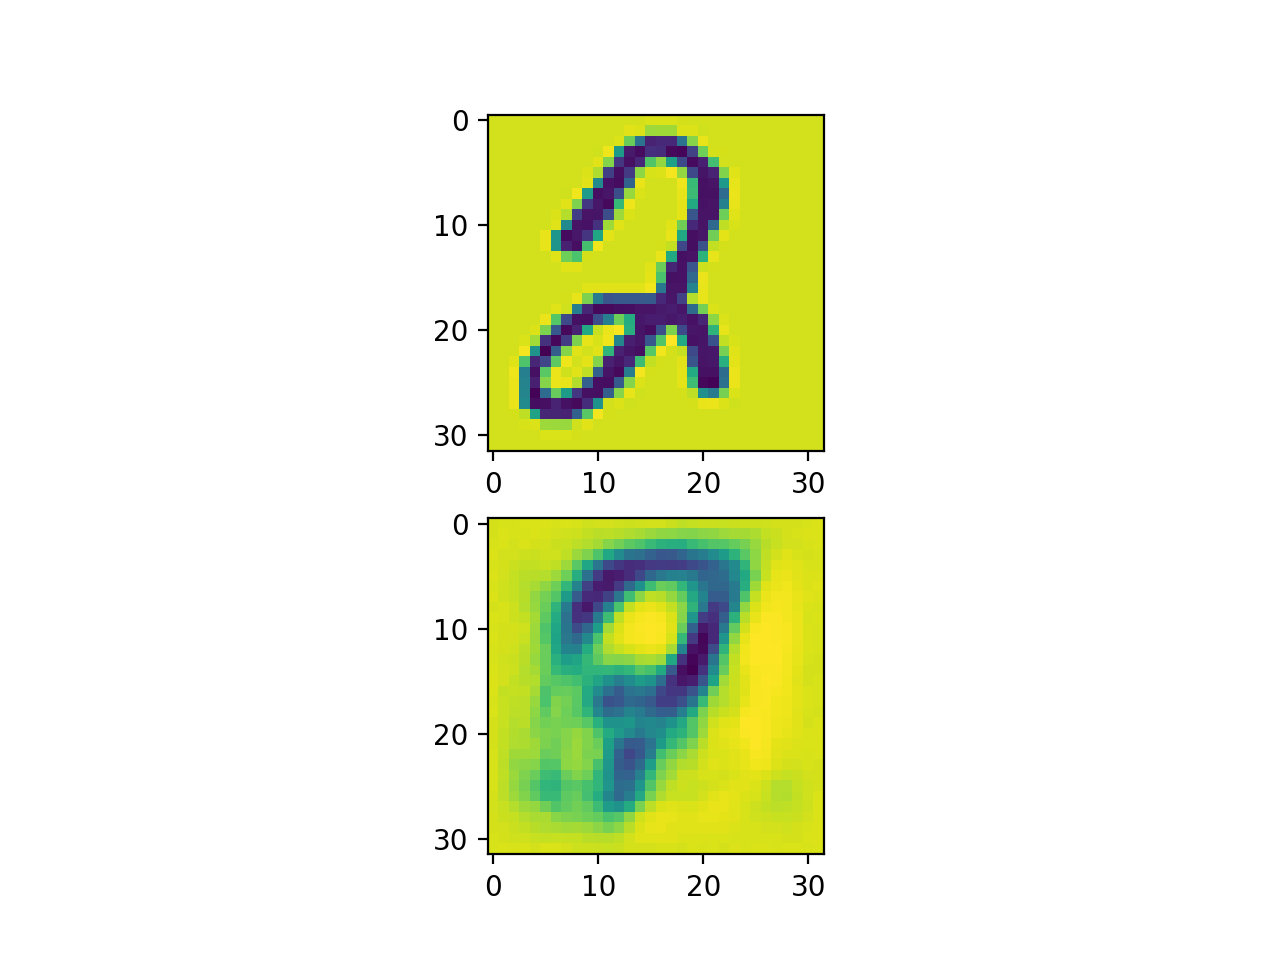
\includegraphics[width=0.4\textwidth]{results/q5_3_22.png}}
\caption{Class 2}
\end{figure}

Class $\mathrm{A}$:
\begin{figure}[H]
\centering
\subfigure[]{
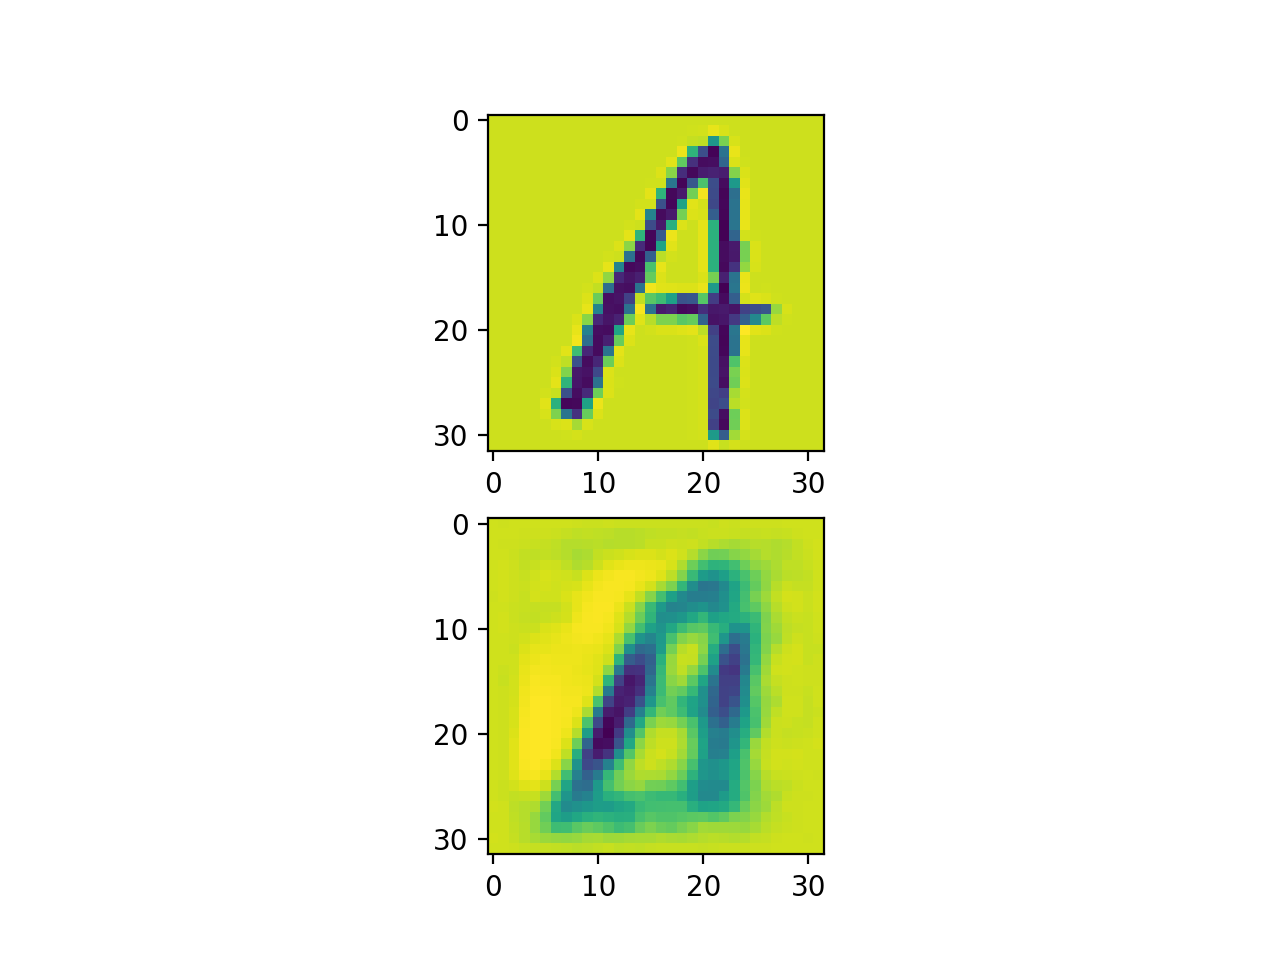
\includegraphics[width=0.4\textwidth]{results/q5_3_a1.png}}
\subfigure[]{
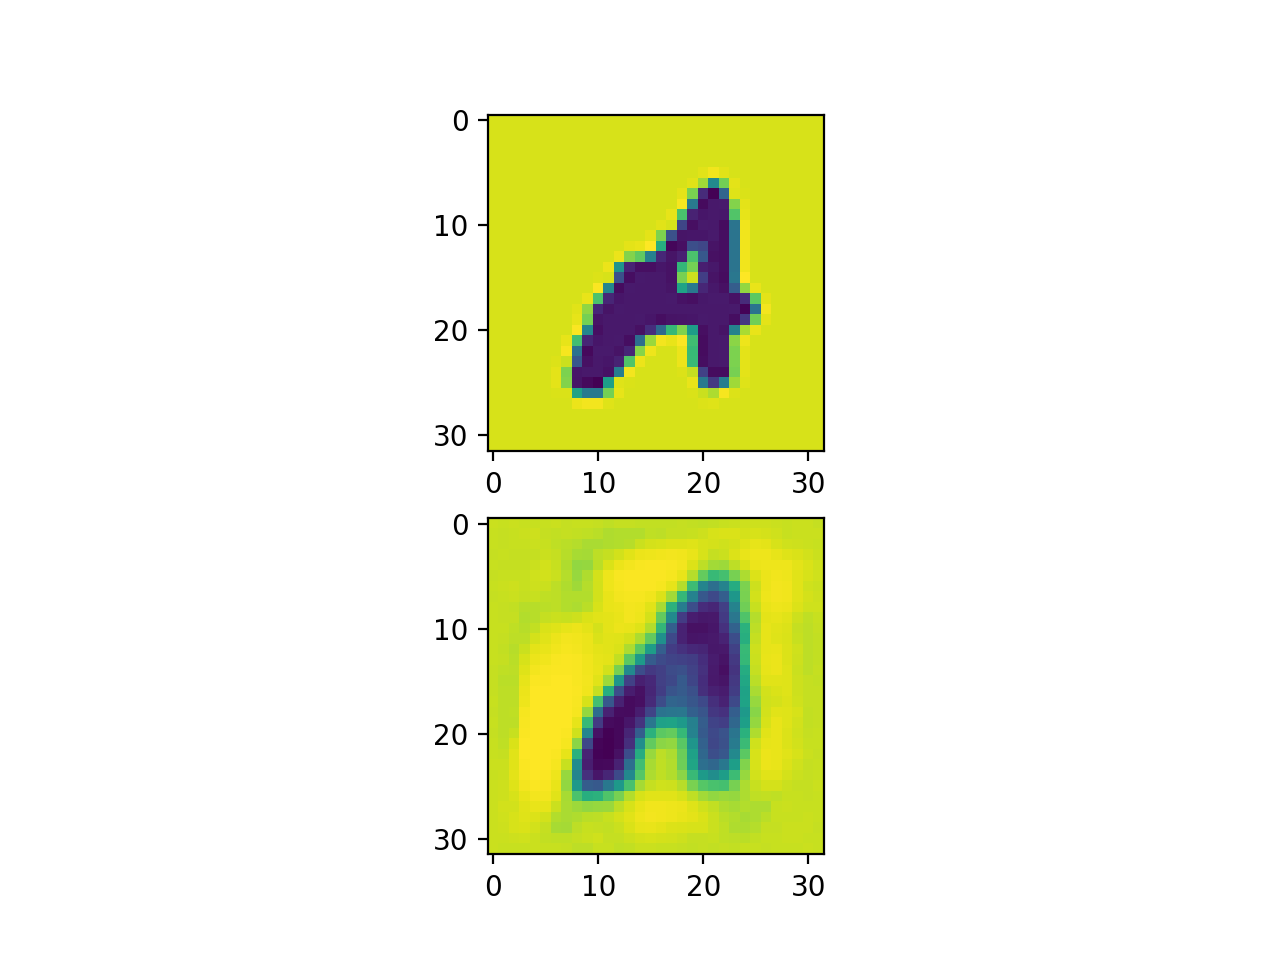
\includegraphics[width=0.4\textwidth]{results/q5_3_a2.png}}
\caption{Class A}
\end{figure}

Class $\mathrm{H}$:
\begin{figure}[H]
\centering
\subfigure[]{
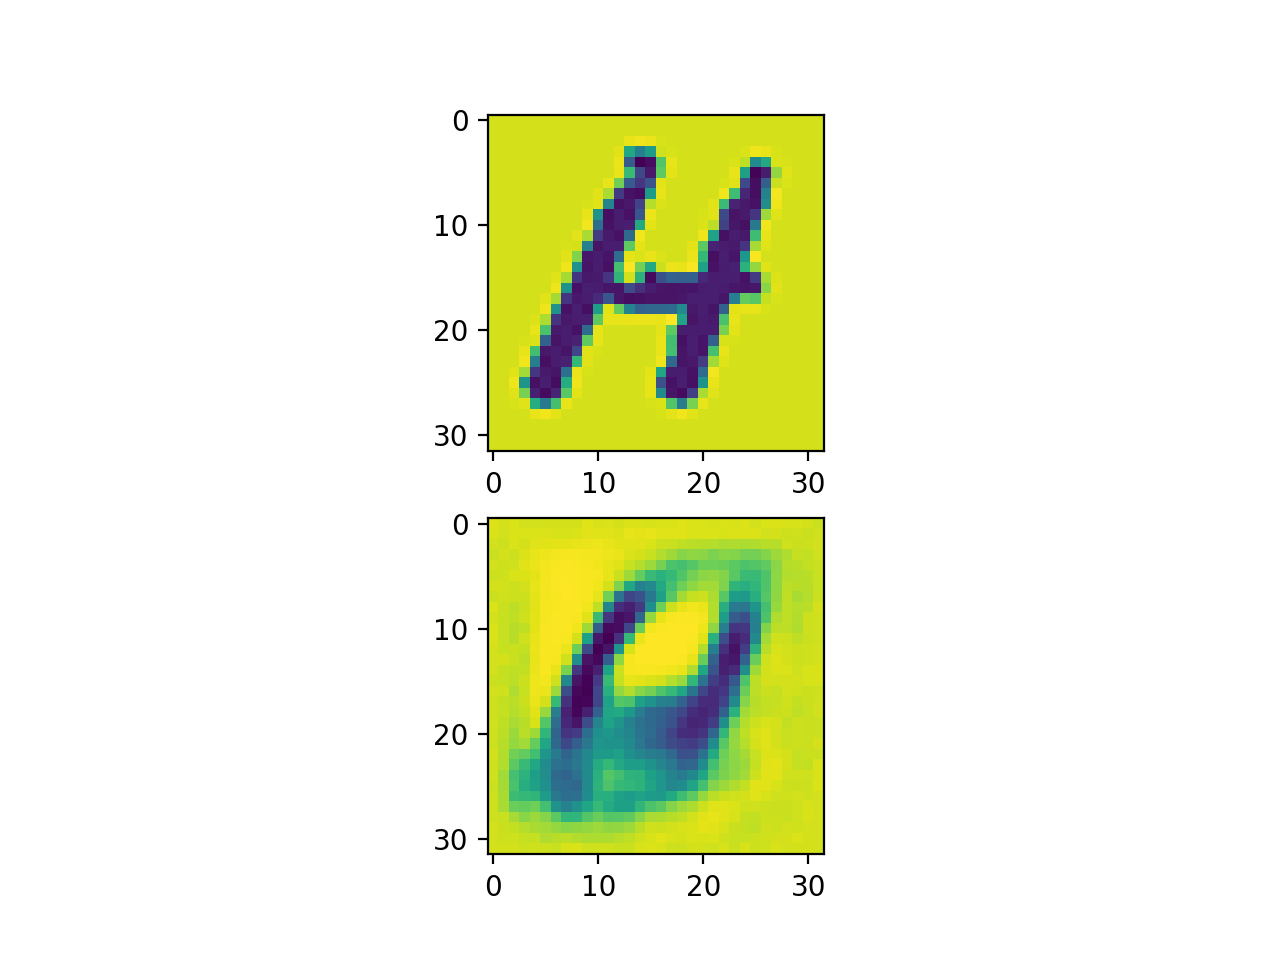
\includegraphics[width=0.4\textwidth]{results/q5_3_h1.png}}
\subfigure[]{
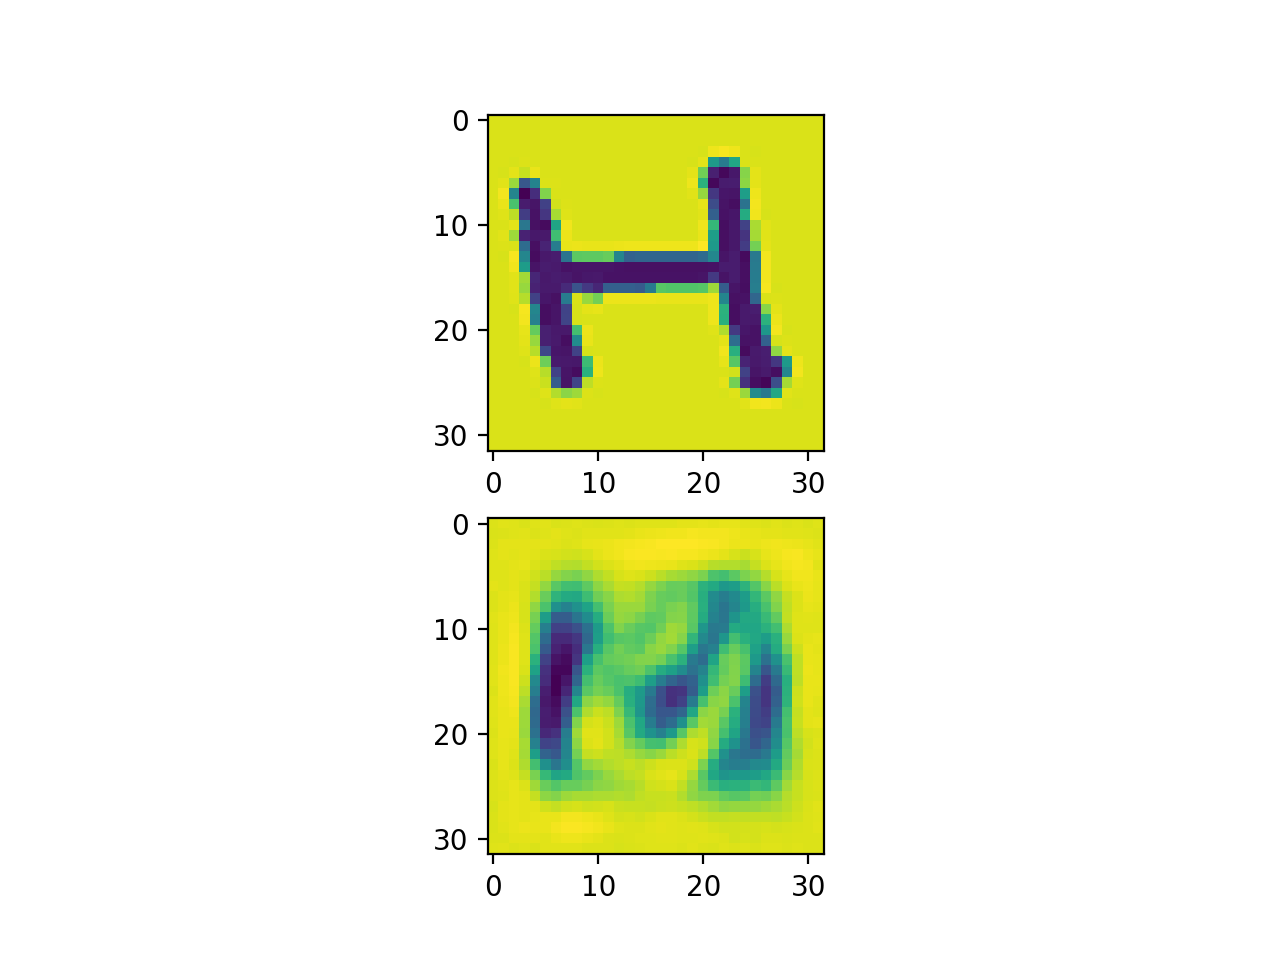
\includegraphics[width=0.4\textwidth]{results/q5_3_h2.png}}
\caption{Class H}
\end{figure}

Class $\mathrm{O}$:
\begin{figure}[H]
\centering
\subfigure[]{
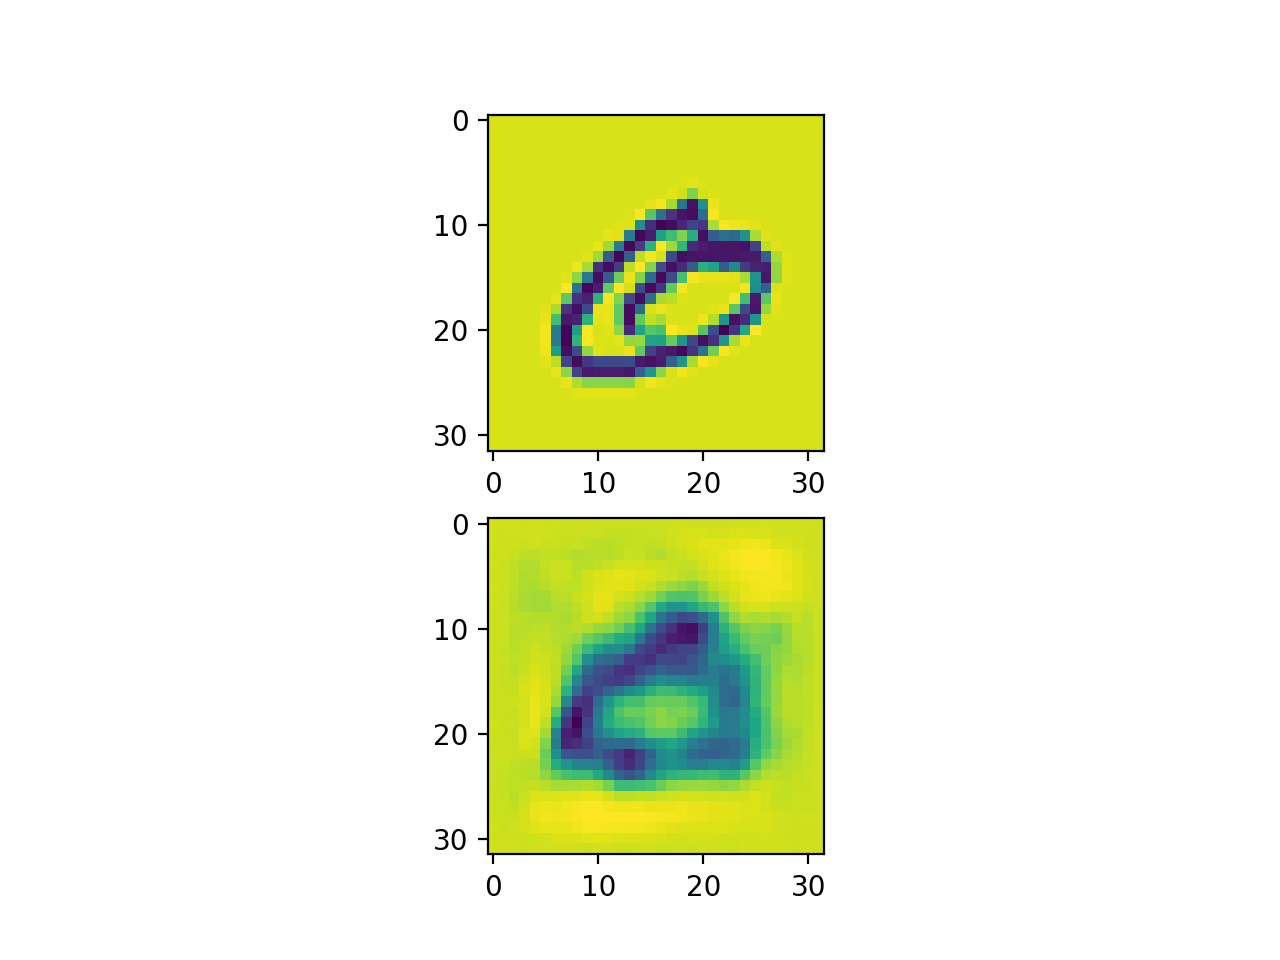
\includegraphics[width=0.4\textwidth]{results/q5_3_o1.png}}
\subfigure[]{
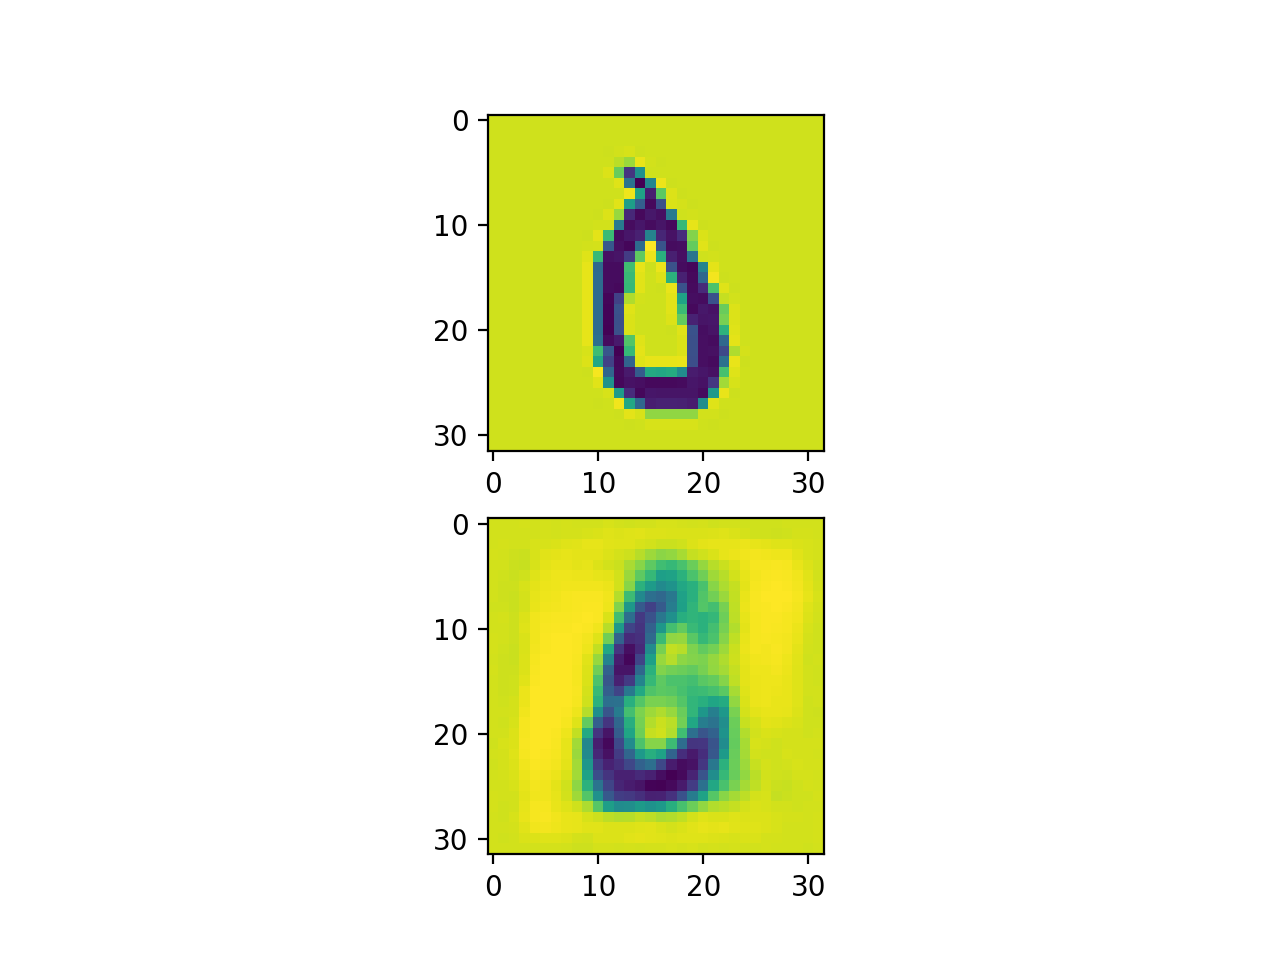
\includegraphics[width=0.4\textwidth]{results/q5_3_o2.png}}
\caption{Class O}
\end{figure}

Class $\mathrm{V}$:
\begin{figure}[H]
\centering
\subfigure[]{
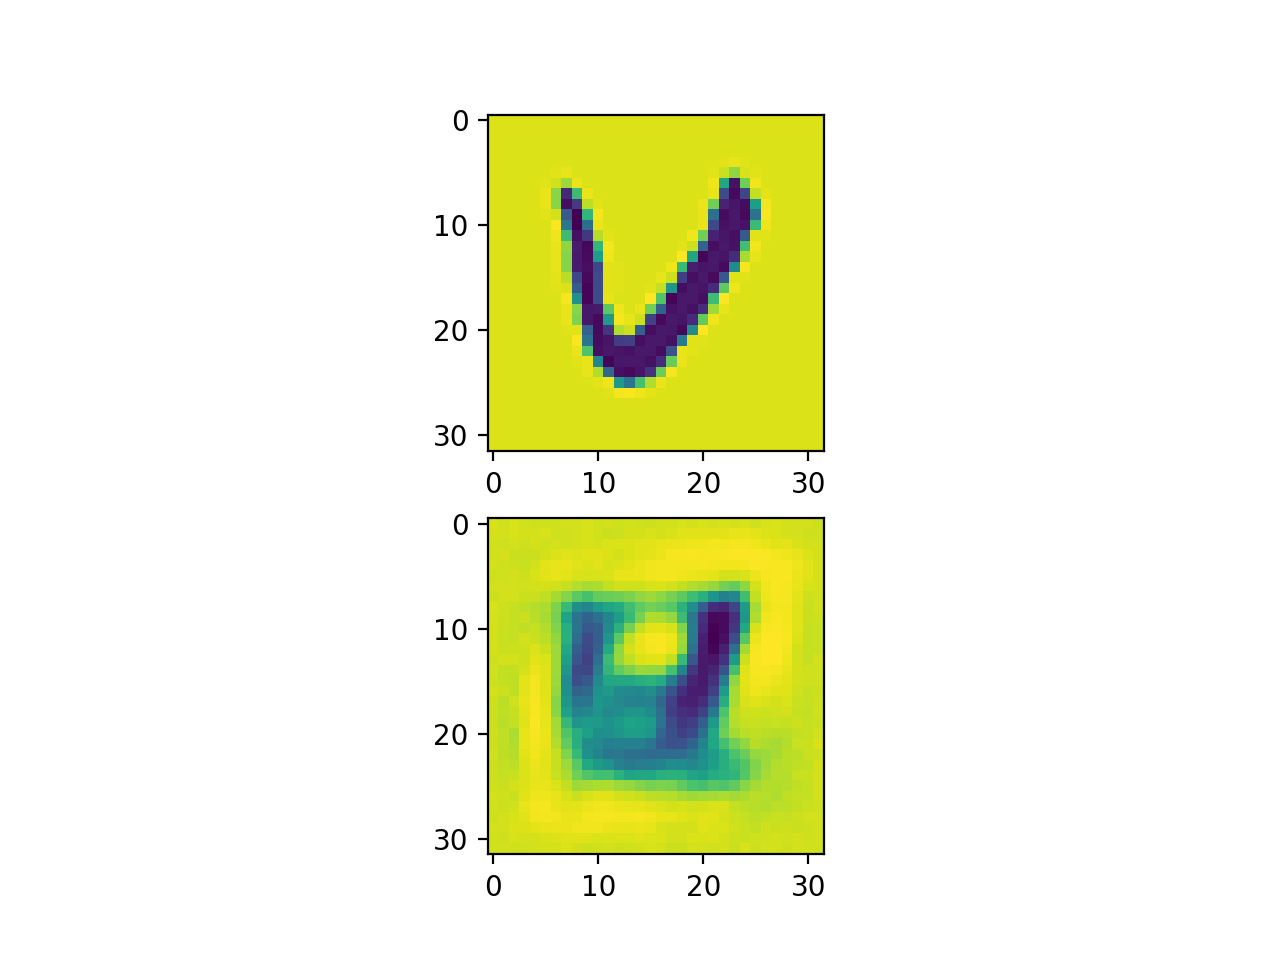
\includegraphics[width=0.4\textwidth]{results/q5_3_v1.png}}
\subfigure[]{
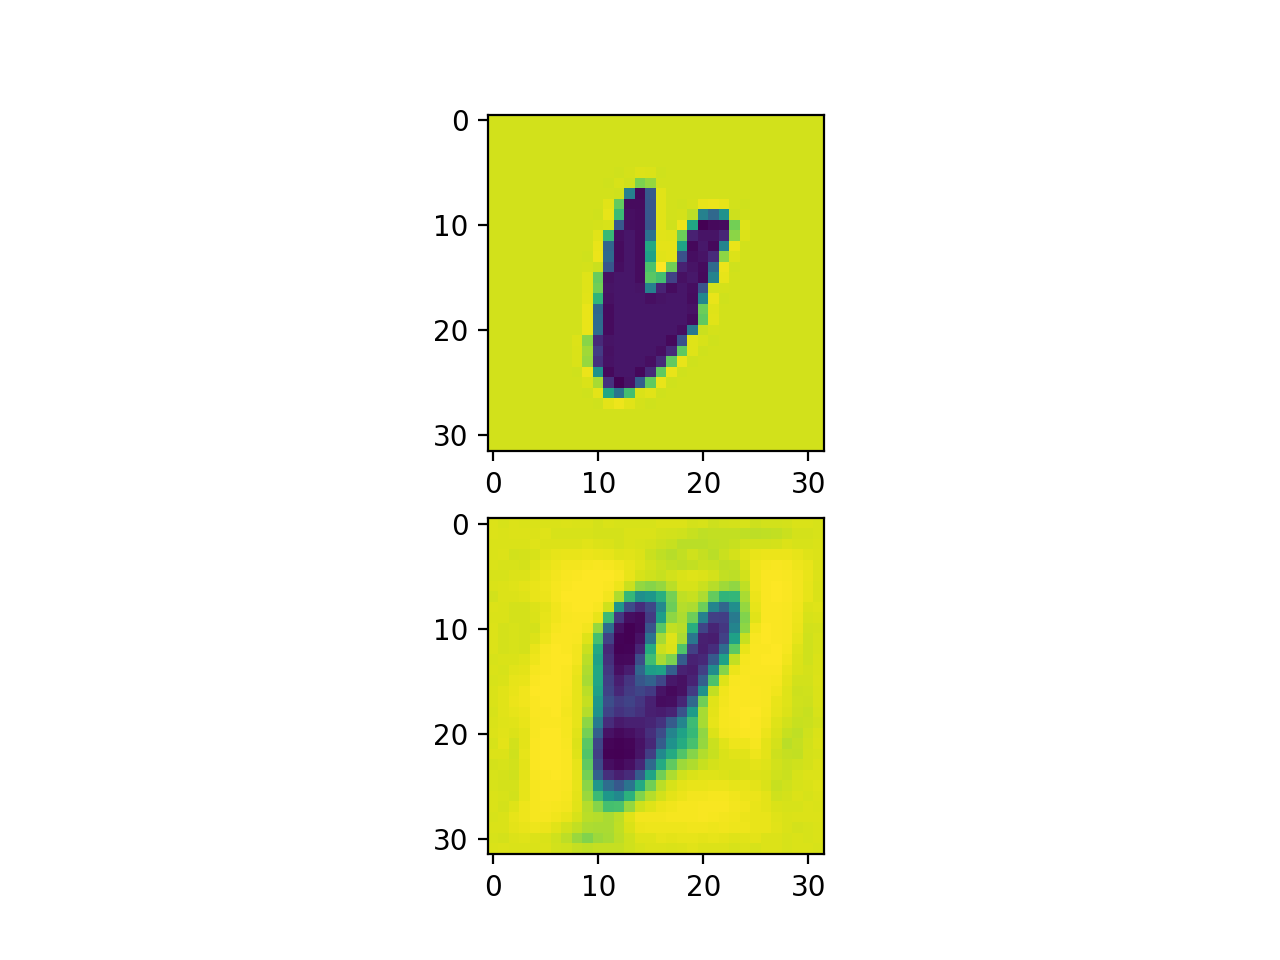
\includegraphics[width=0.4\textwidth]{results/q5_3_v2.png}}
\caption{Class V}
\end{figure}

We could approximately tell the shapes of reconstructed figures are quite similar to the original ones, but autoencoder is unable to fully reconstruct the figure, so the reconstructed figures are blurred.

\paragraph{Q5.3.2}~{}

With default settings and batch size $36$, learning rate $3e-5$, the $\mathrm{PSNR}$ is $13.52373364094888$.

\section{PyTorch}
\subsection{Train a Neural Network in PyTorch}
\paragraph{Q6.1.1}~{}

\begin{figure}[H]
\centering
\subfigure[Loss Figure]{
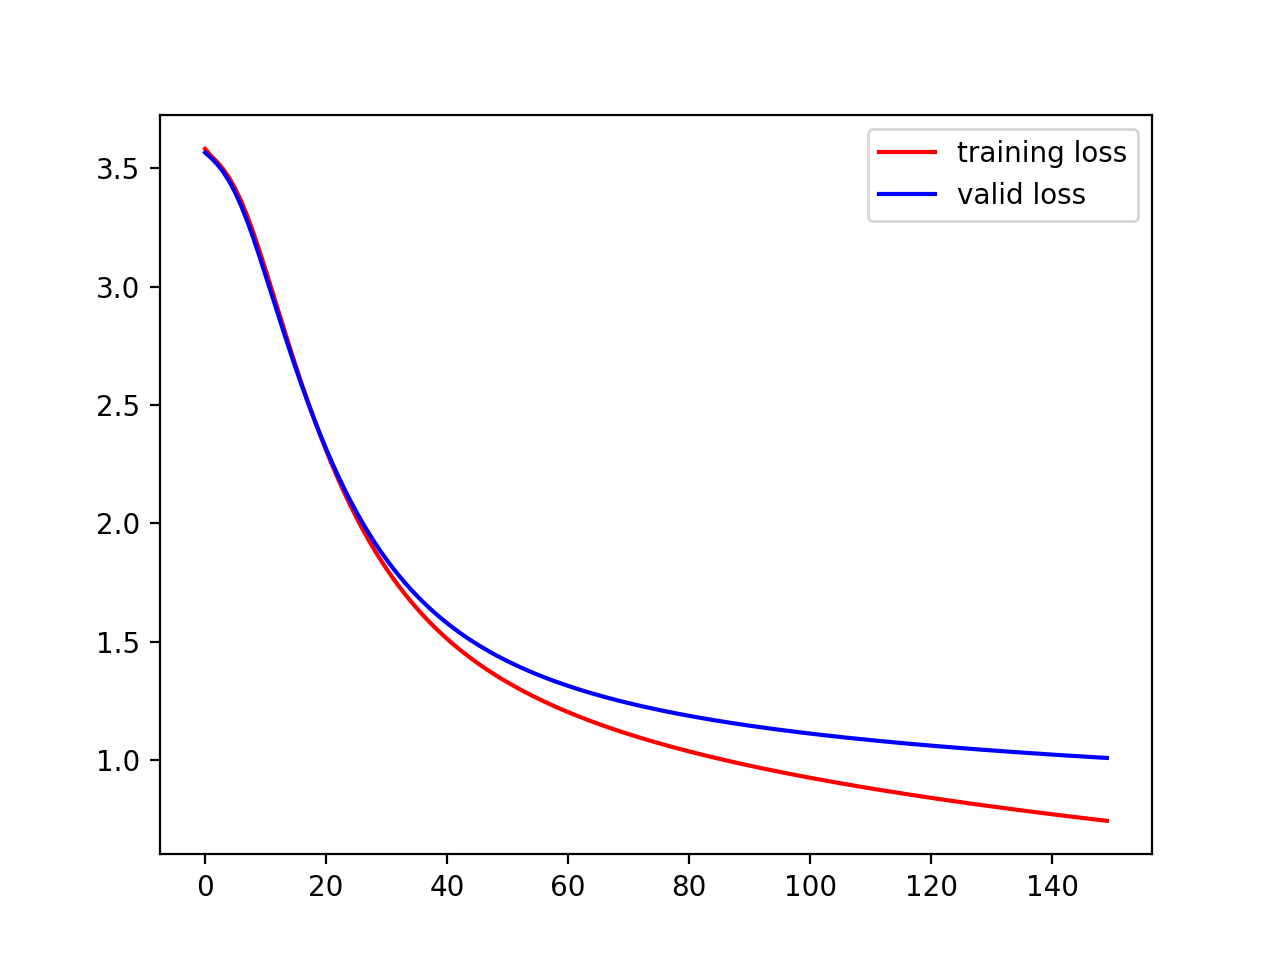
\includegraphics[width=0.4\textwidth]{results/q6_1_1loss.png}}
\subfigure[Accuracy Figure]{
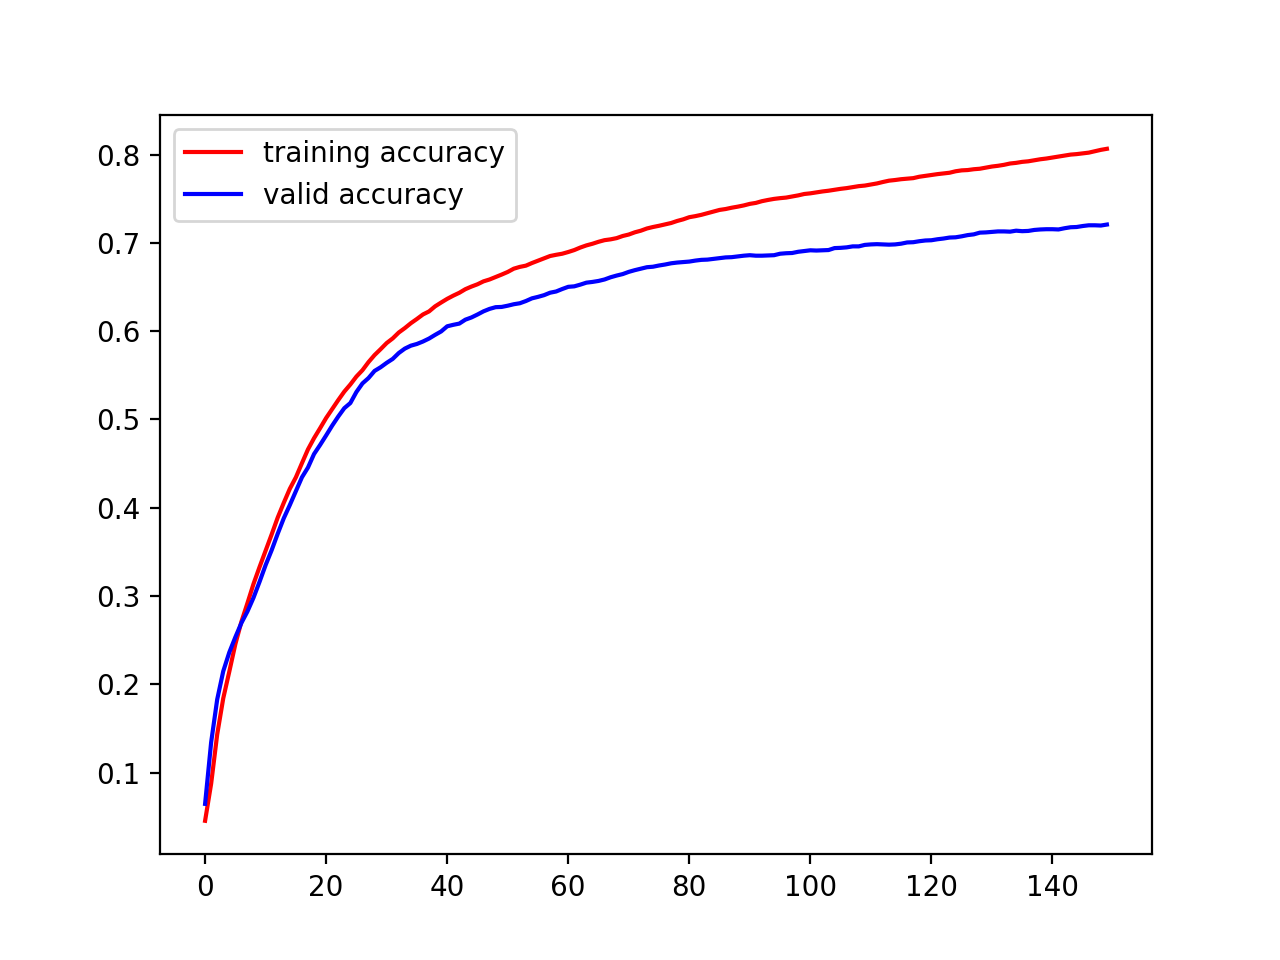
\includegraphics[width=0.4\textwidth]{results/q6_1_1acc.png}}
\caption{Loss and Accuracy Figures}
\end{figure}


\paragraph{Q6.1.2}~{}

The structure of convolutional network is:
\begin{figure}[H]
\centering
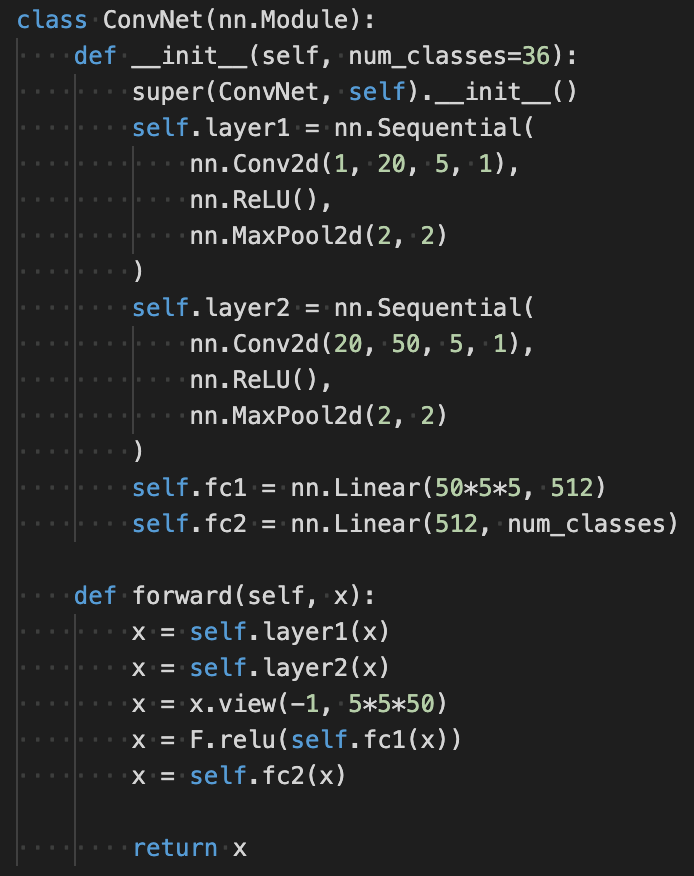
\includegraphics[width=0.5\textwidth]{results/q6_1_2.png}
\caption{Network Structure}
\end{figure}
and the results are shown below:

\begin{figure}[H]
\centering
\subfigure[Loss Figure]{
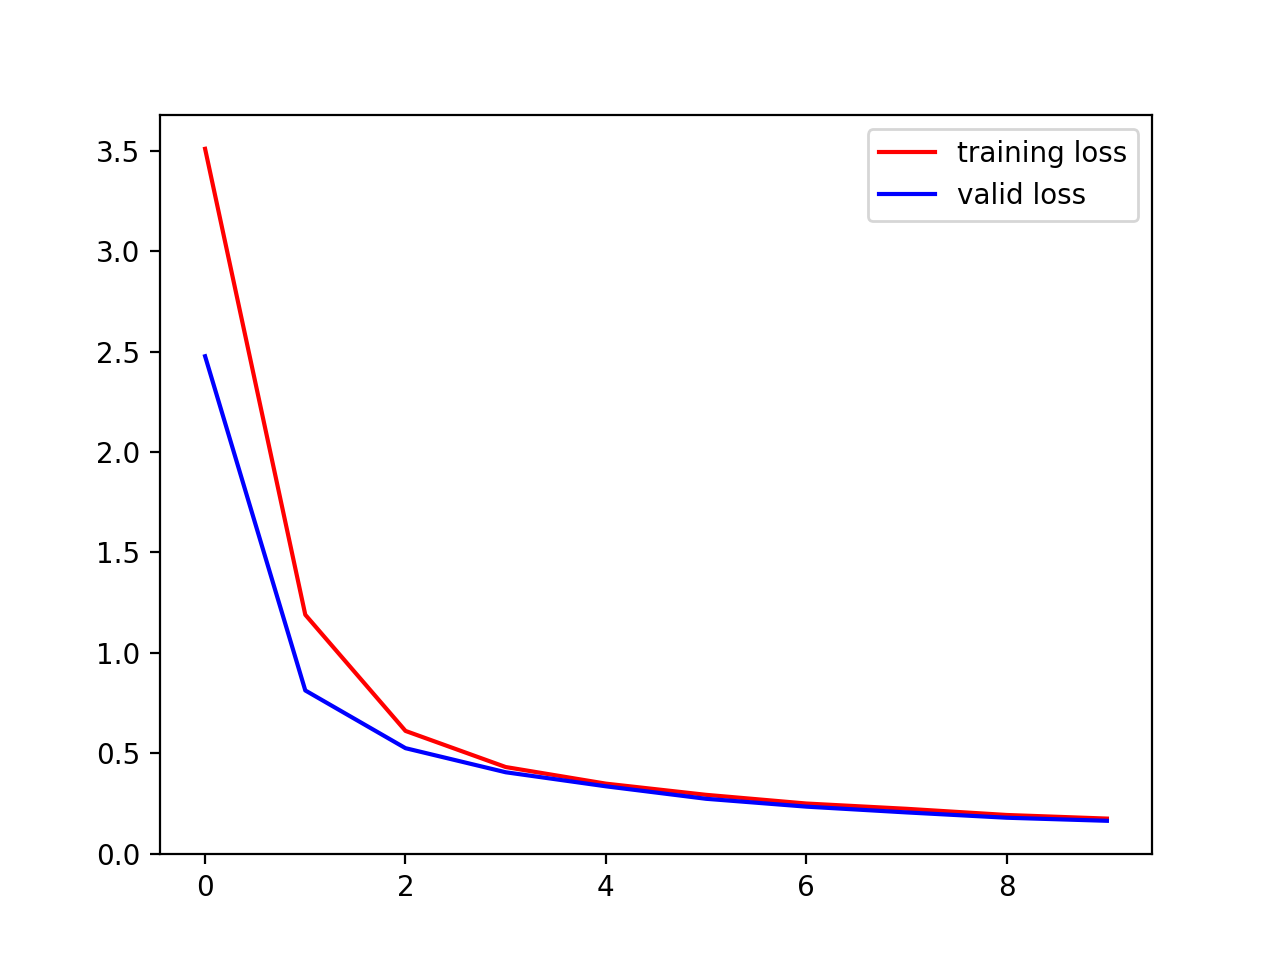
\includegraphics[width=0.4\textwidth]{results/q6_1_2loss.png}}
\subfigure[Accuracy Figure]{
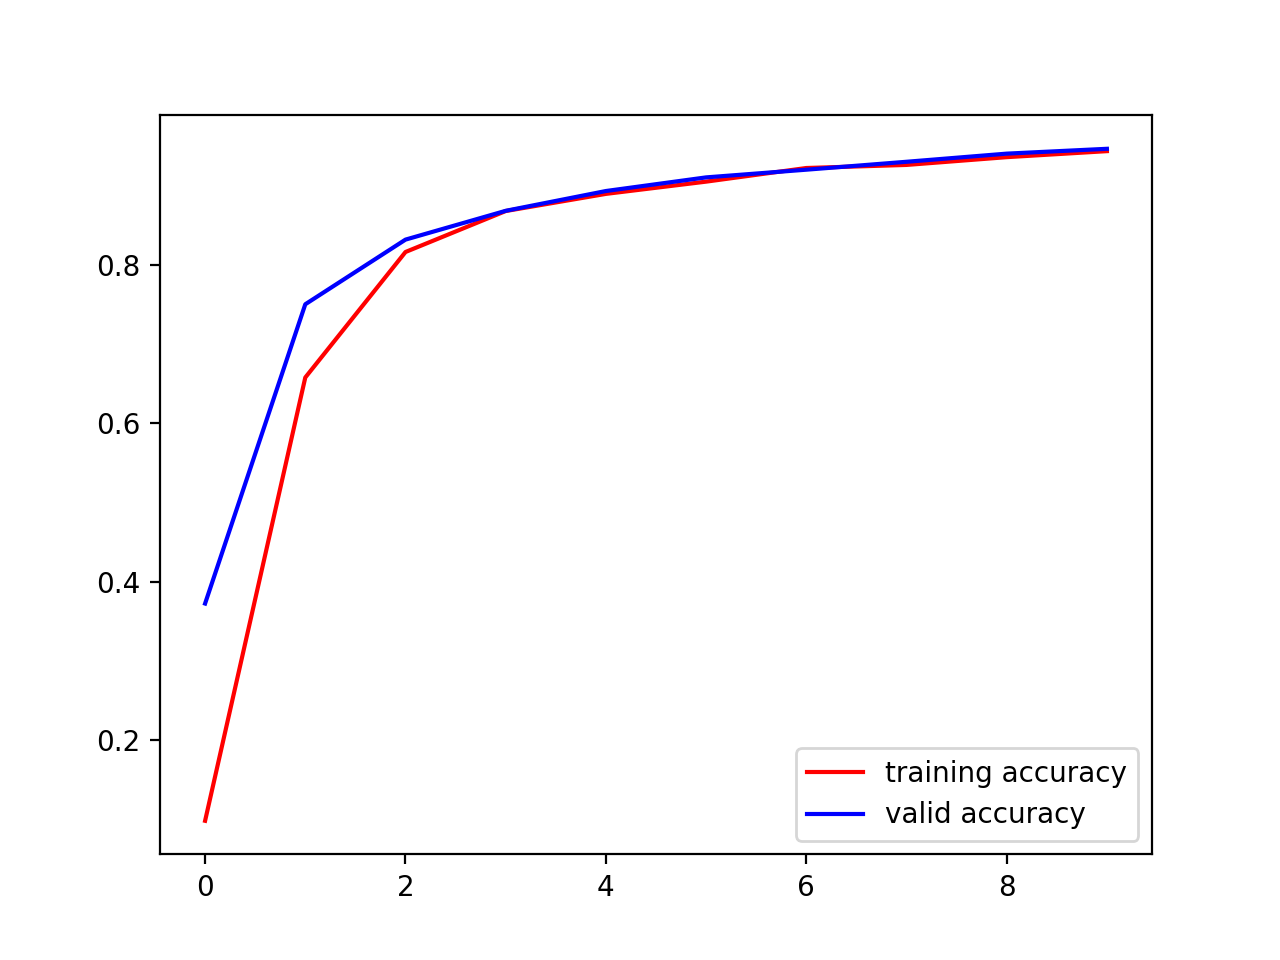
\includegraphics[width=0.4\textwidth]{results/q6_1_2acc.png}}
\caption{Loss and Accuracy Figures}
\end{figure}

Compared with the fully-connected network, the convolutional network converged faster and reached a significantly higher accuracy, and the loss in convolutional network dropped sharply at the first two iterations.

\end{document}
